\documentclass[12pt]{article}


\usepackage{amssymb}
\usepackage{amsmath}
\usepackage{fullpage}
\usepackage{epsfig}
\usepackage{epstopdf}
\everymath{\displaystyle}
\usepackage{enumerate}



\begin{document}

\begin{center}
\underline{\LARGE{Multivariable Functions}}
\end{center}

\noindent SUGGESTED REFERENCE MATERIAL:

\bigskip

\noindent As you work through the problems listed below, you should reference Chapter 13.1 of the recommended textbook (or the equivalent chapter in your alternative textbook/online resource) and your lecture notes.

\noindent EXPECTED SKILLS:

\begin{itemize}

\item Be able to describe and sketch the domain of a function of two or more variables.

\item Know how to evaluate a function of two or more variables.

\item Be able to compute and sketch level curves \& surfaces.

\end{itemize}

\noindent PRACTICE PROBLEMS:

\medskip

\begin{enumerate}

\item For each of the following functions, describe the domain in words.  Whenever possible, draw a sketch of the domain as well.

\begin{enumerate}

\item $f(x,y)=\sqrt{10-x^2-y^2}$

\includegraphics[scale=0.5]{start.pdf}
{{{1\linewidth}{The domain is all points in the $xy$-plane which are on or inside of $x^2+y^2=10$, the circle with a radius of $\sqrt{10}$ centered at the origin.
\begin{center}
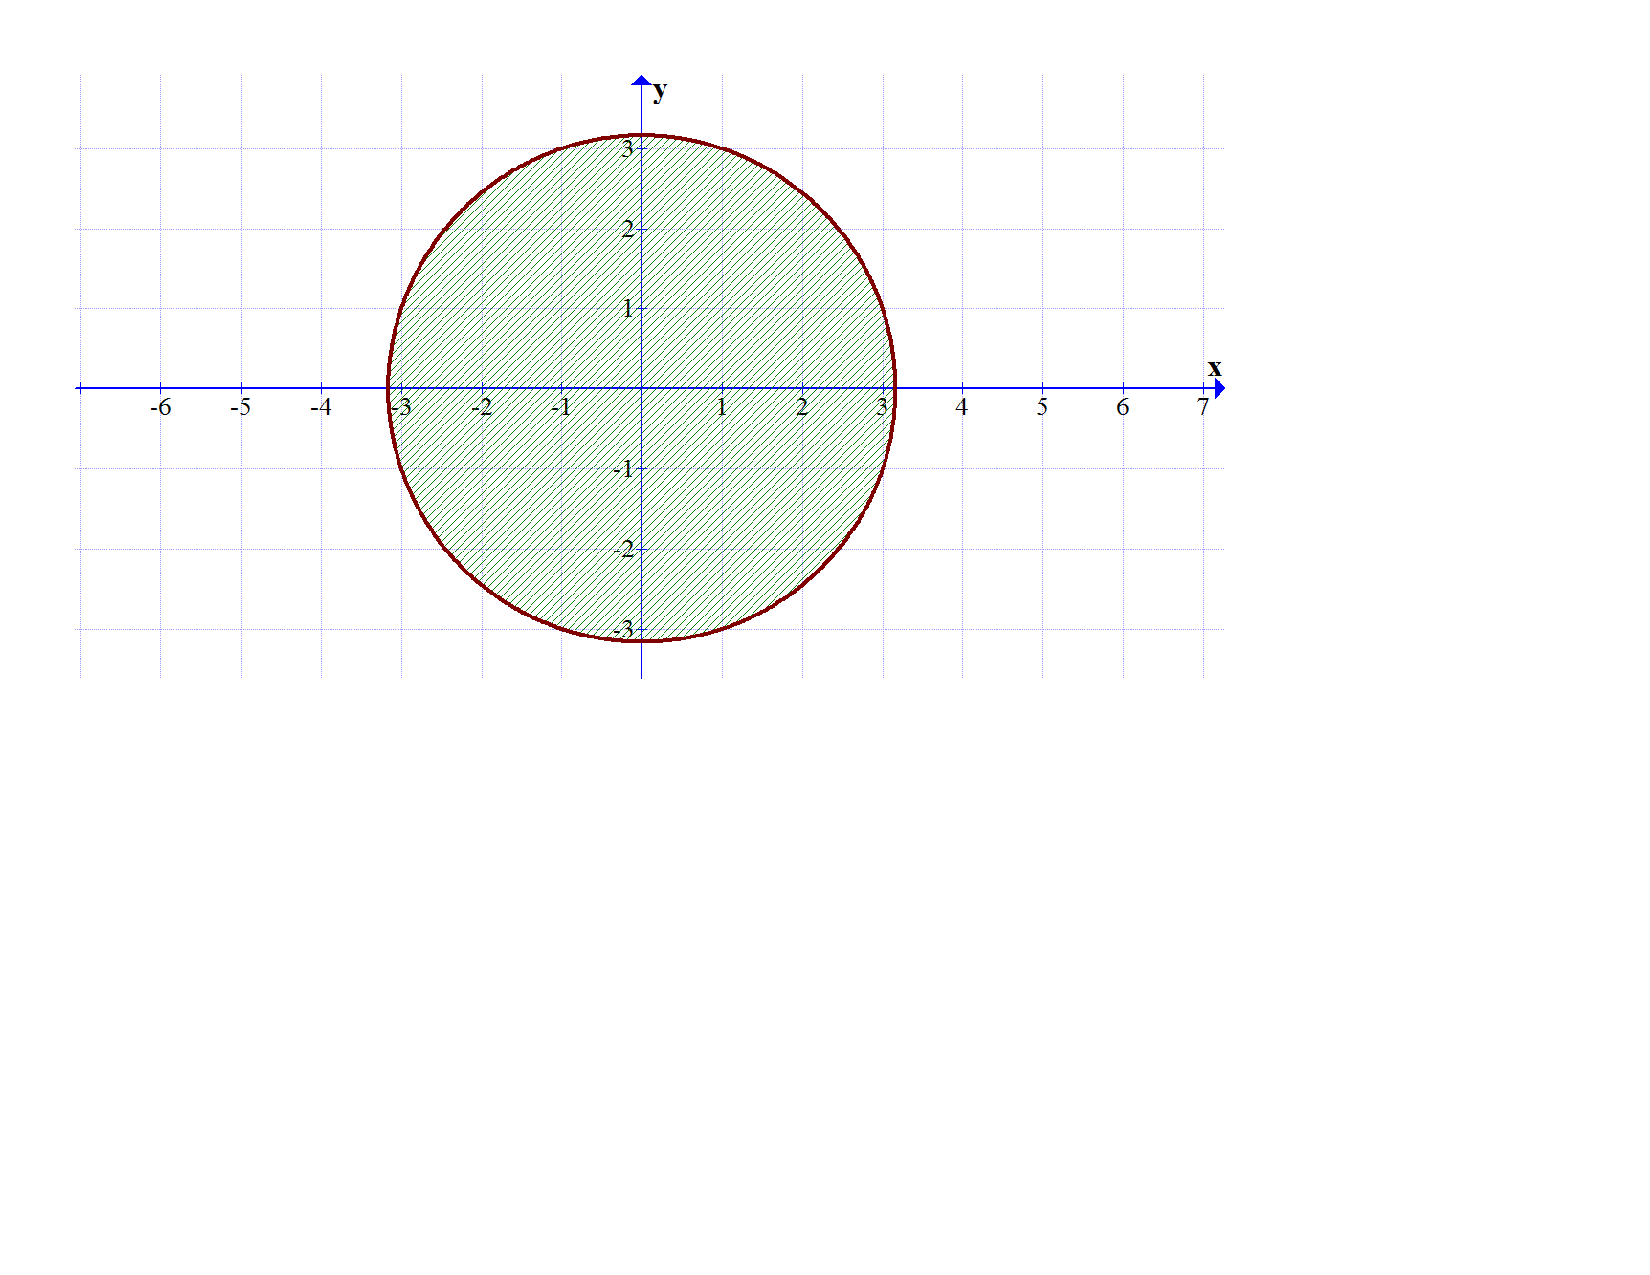
\includegraphics[scale=0.4]{domain1.pdf}
\end{center}}}}
\includegraphics[scale=0.5]{end.pdf}


\item $f(x,y)=\arcsin{(2x+y)}$

\includegraphics[scale=0.5]{start.pdf}
{{{1\linewidth}{The domain is all points in the $xy$ plane which are between the lines $y=-2x-1$ and $y=-2x+1$, including the points on the lines.\\
\begin{center}
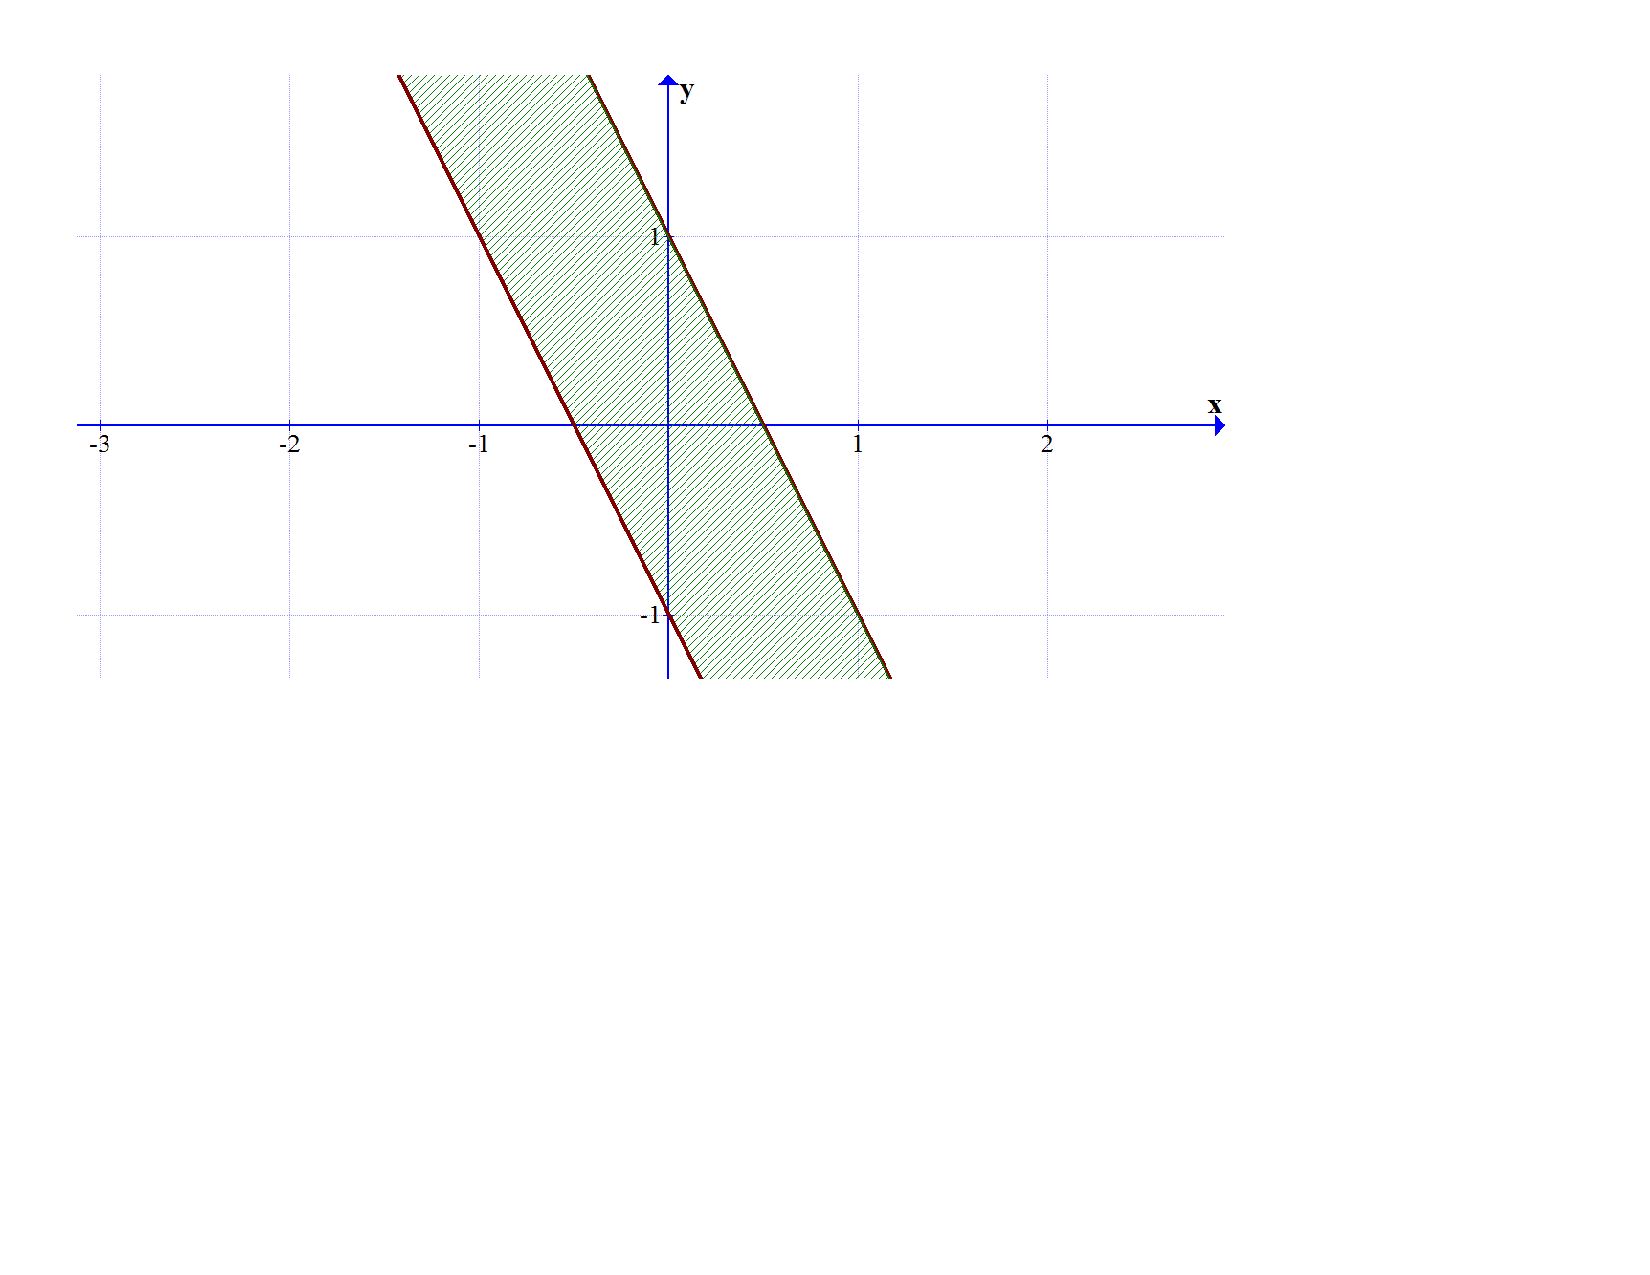
\includegraphics[scale=0.4]{domain2.pdf}
\end{center}}}}
\includegraphics[scale=0.5]{end.pdf}


\item $f(x,y,z)=\ln{(36-4x^2-9y^2-36z^2)}$

\includegraphics[scale=0.5]{start.pdf}
{{{1\linewidth}{All point in 3-space which are inside of (but not on) the ellipsoid $\frac{x^2}{9}+\frac{y^2}{4}+z^2=1$.
\begin{center}
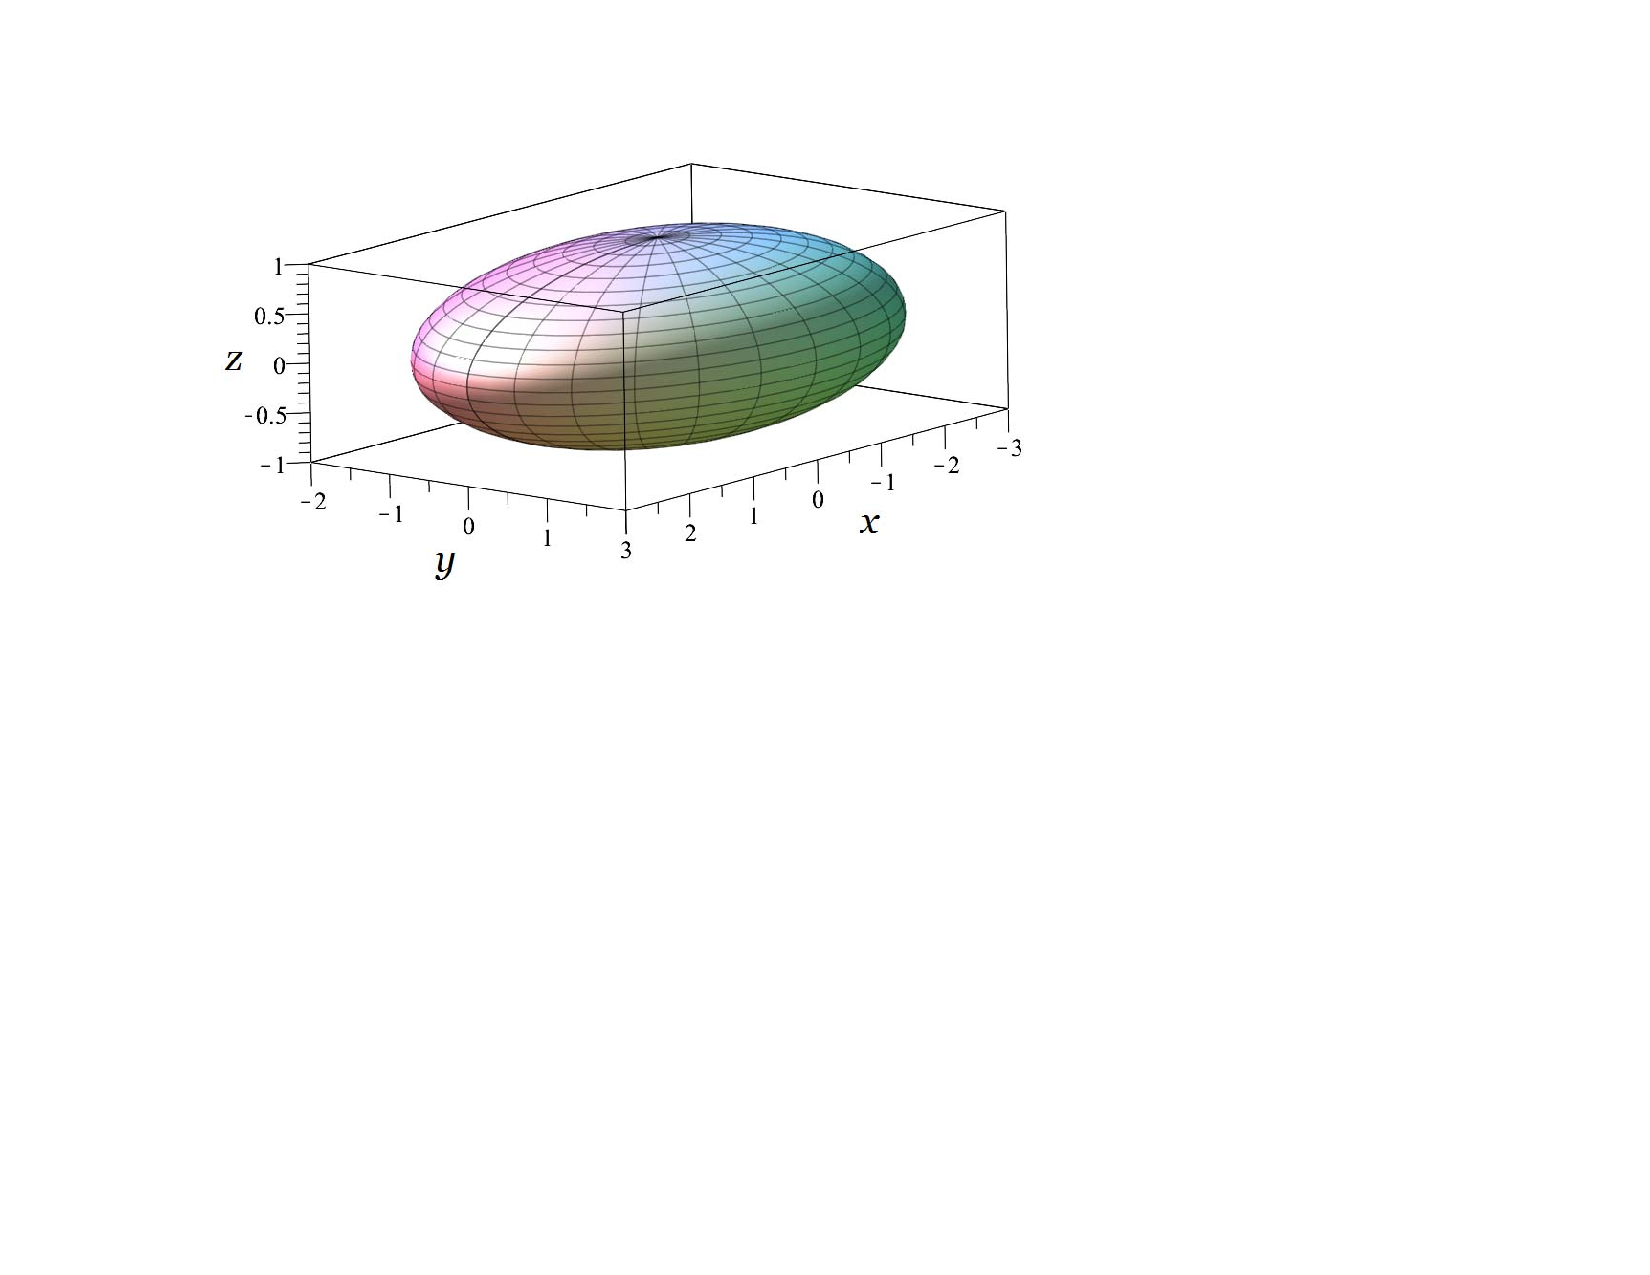
\includegraphics[scale=0.4]{domain3.pdf}
\end{center}}}}
\includegraphics[scale=0.5]{end.pdf}


\item $f(x,y,z)=\sqrt{6-2x-3y-z}$

\includegraphics[scale=0.5]{start.pdf}
{{All points in 3-space which are on or below the plane $2x+3y+z=6$}}
\includegraphics[scale=0.5]{end.pdf}


\end{enumerate}

\item Let $f(x,y)=2xe^{3y}$.  Compute the following.

\begin{enumerate}

\item $f(4,0)$

\includegraphics[scale=0.5]{start.pdf}
{{8}}
\includegraphics[scale=0.5]{end.pdf}


\item $f(1,\ln2)$

\includegraphics[scale=0.5]{start.pdf}
{{16}}
\includegraphics[scale=0.5]{end.pdf}


\end{enumerate}

\item Suppose $f(x,y)=\int_x^y (t^2-1) \,dt$.  Compute the following.

\begin{enumerate}

\item $f(-1,2)$

\includegraphics[scale=0.5]{start.pdf}
{{0}}
\includegraphics[scale=0.5]{end.pdf}


\item $f(0,2)$

\includegraphics[scale=0.5]{start.pdf}
{{$\frac{2}{3}$}}
\includegraphics[scale=0.5]{end.pdf}


\end{enumerate}

\item Suppose $f(x_1,x_2,\dots,x_n)=x_1+2x_2+3x_3+\dots+nx_n$.  Determine $f(1,1,\dots,1)$.

\includegraphics[scale=0.5]{start.pdf}
{{$\frac{n(n+1)}{2}$}}
\includegraphics[scale=0.5]{end.pdf}


\item Consider $f(x,y)=x^2+y^2$.  Compute $f(x(t),y(t))$ if $x(t)=1+t$ and $y(t)=2-3t$

\includegraphics[scale=0.5]{start.pdf}
{{$10t^2-10t+5$}}
\includegraphics[scale=0.5]{end.pdf}


\newpage

\item Sketch the level curves $f(x,y)=k$, for the specified values of $k$.

\begin{enumerate}

\item $z=2x-y$; $k=-2,-1, 0, 1, 2$ 

\item $z=y^2-x^2$; $k=-2,-1, 0, 1, 2$

\end{enumerate}

\item {\bf Multiple Choice:} Which of the following graphs is the level curve of $\displaystyle f(x,y)=x^{2}+4y^2$ which passes through $P(-2,0)$?
\begin{center}
\begin{tabular}{llll}
(a) & & (d) &\\
&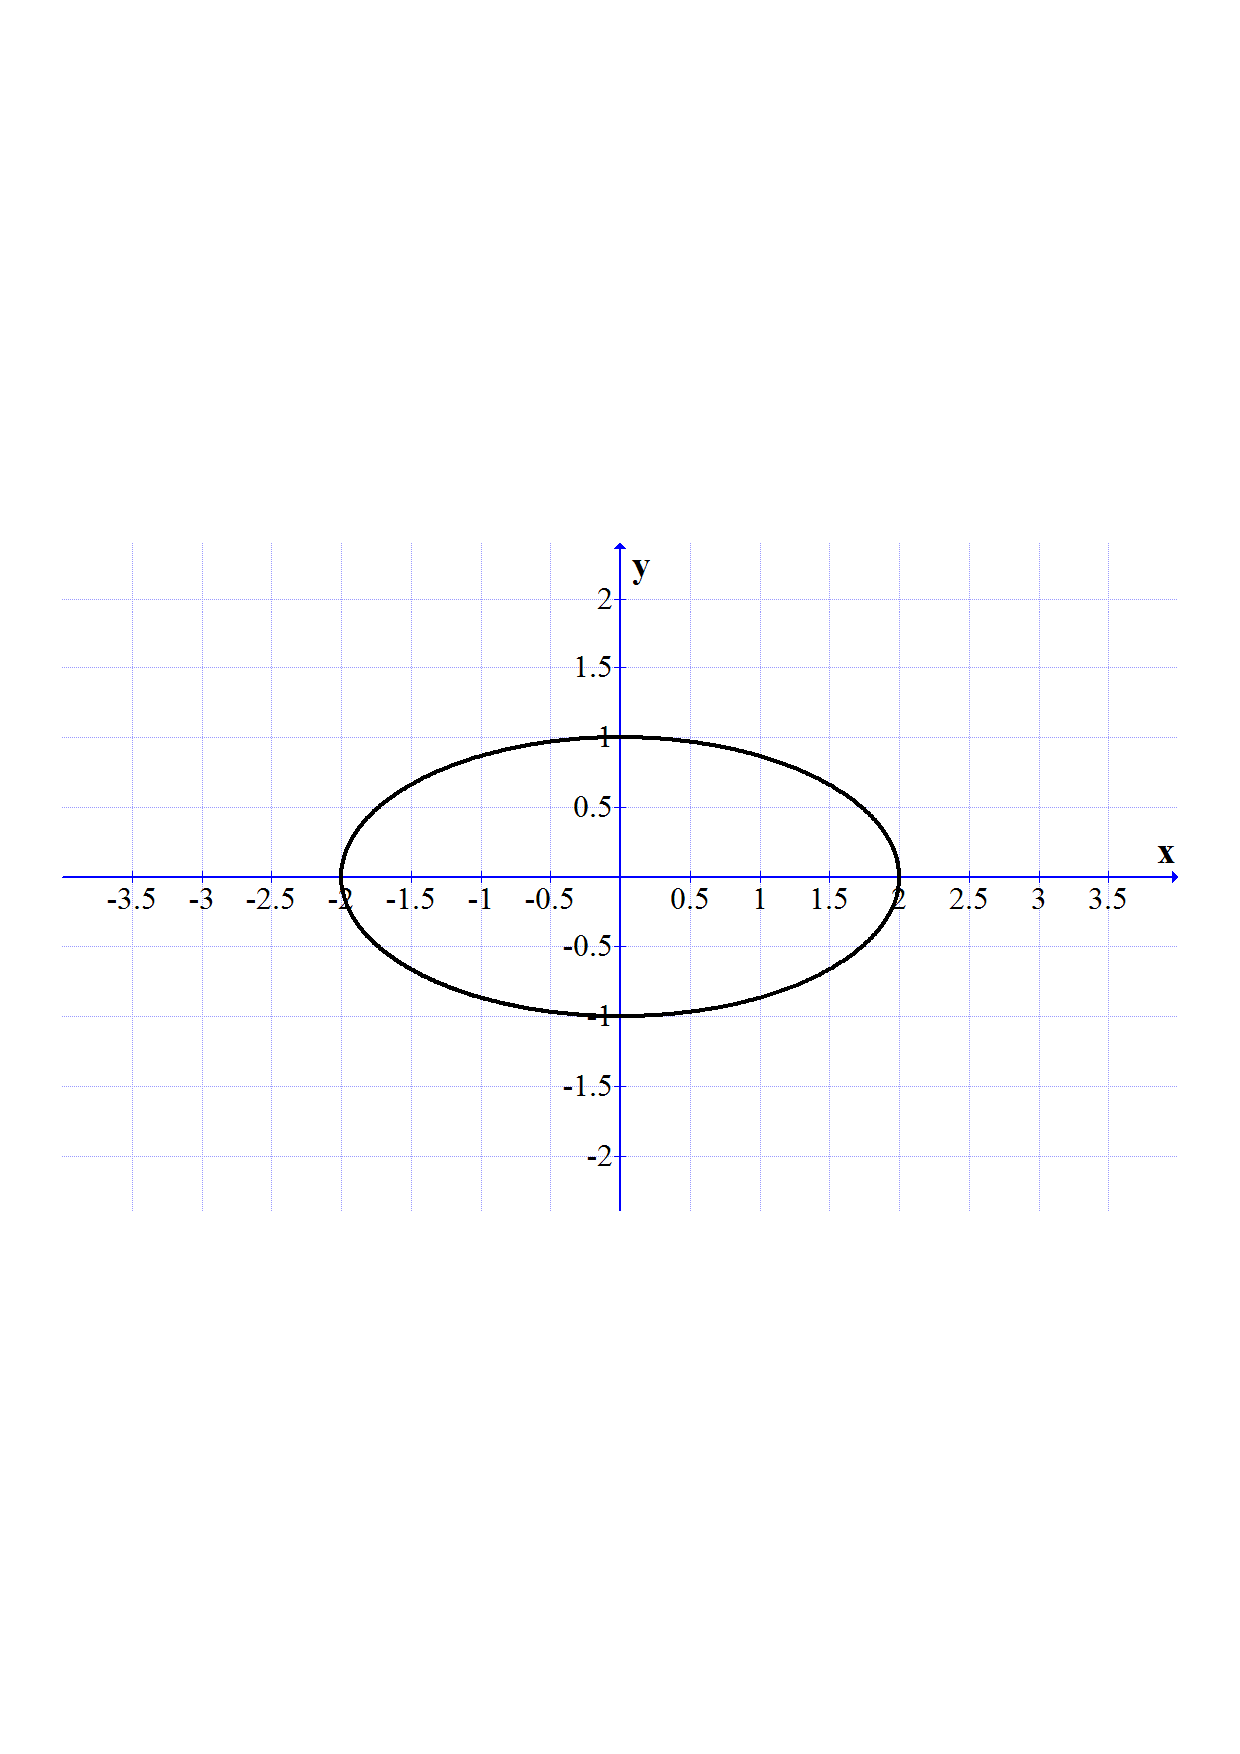
\includegraphics[scale=0.35]{LC1.pdf} & & 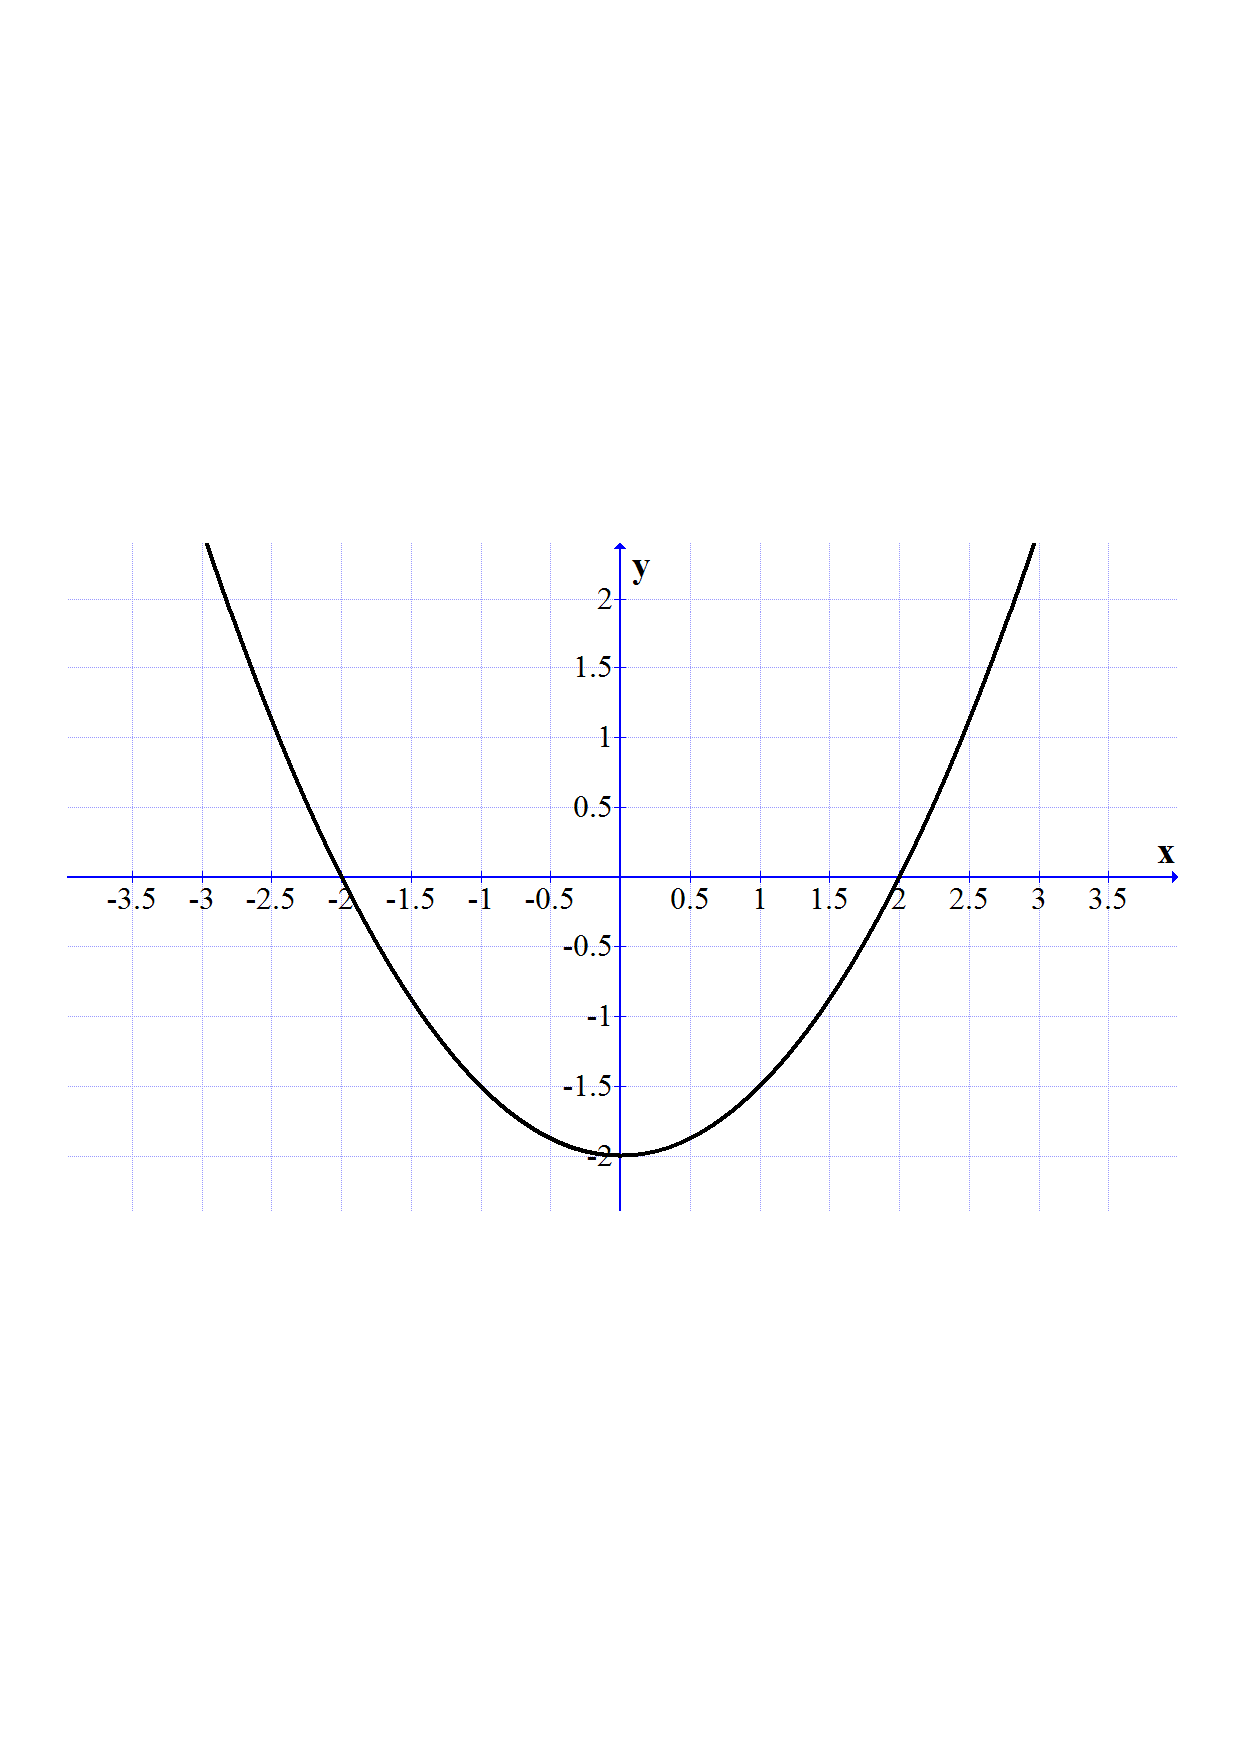
\includegraphics[scale=0.35]{LC4.pdf}\\
(b) & & (e) &\\
&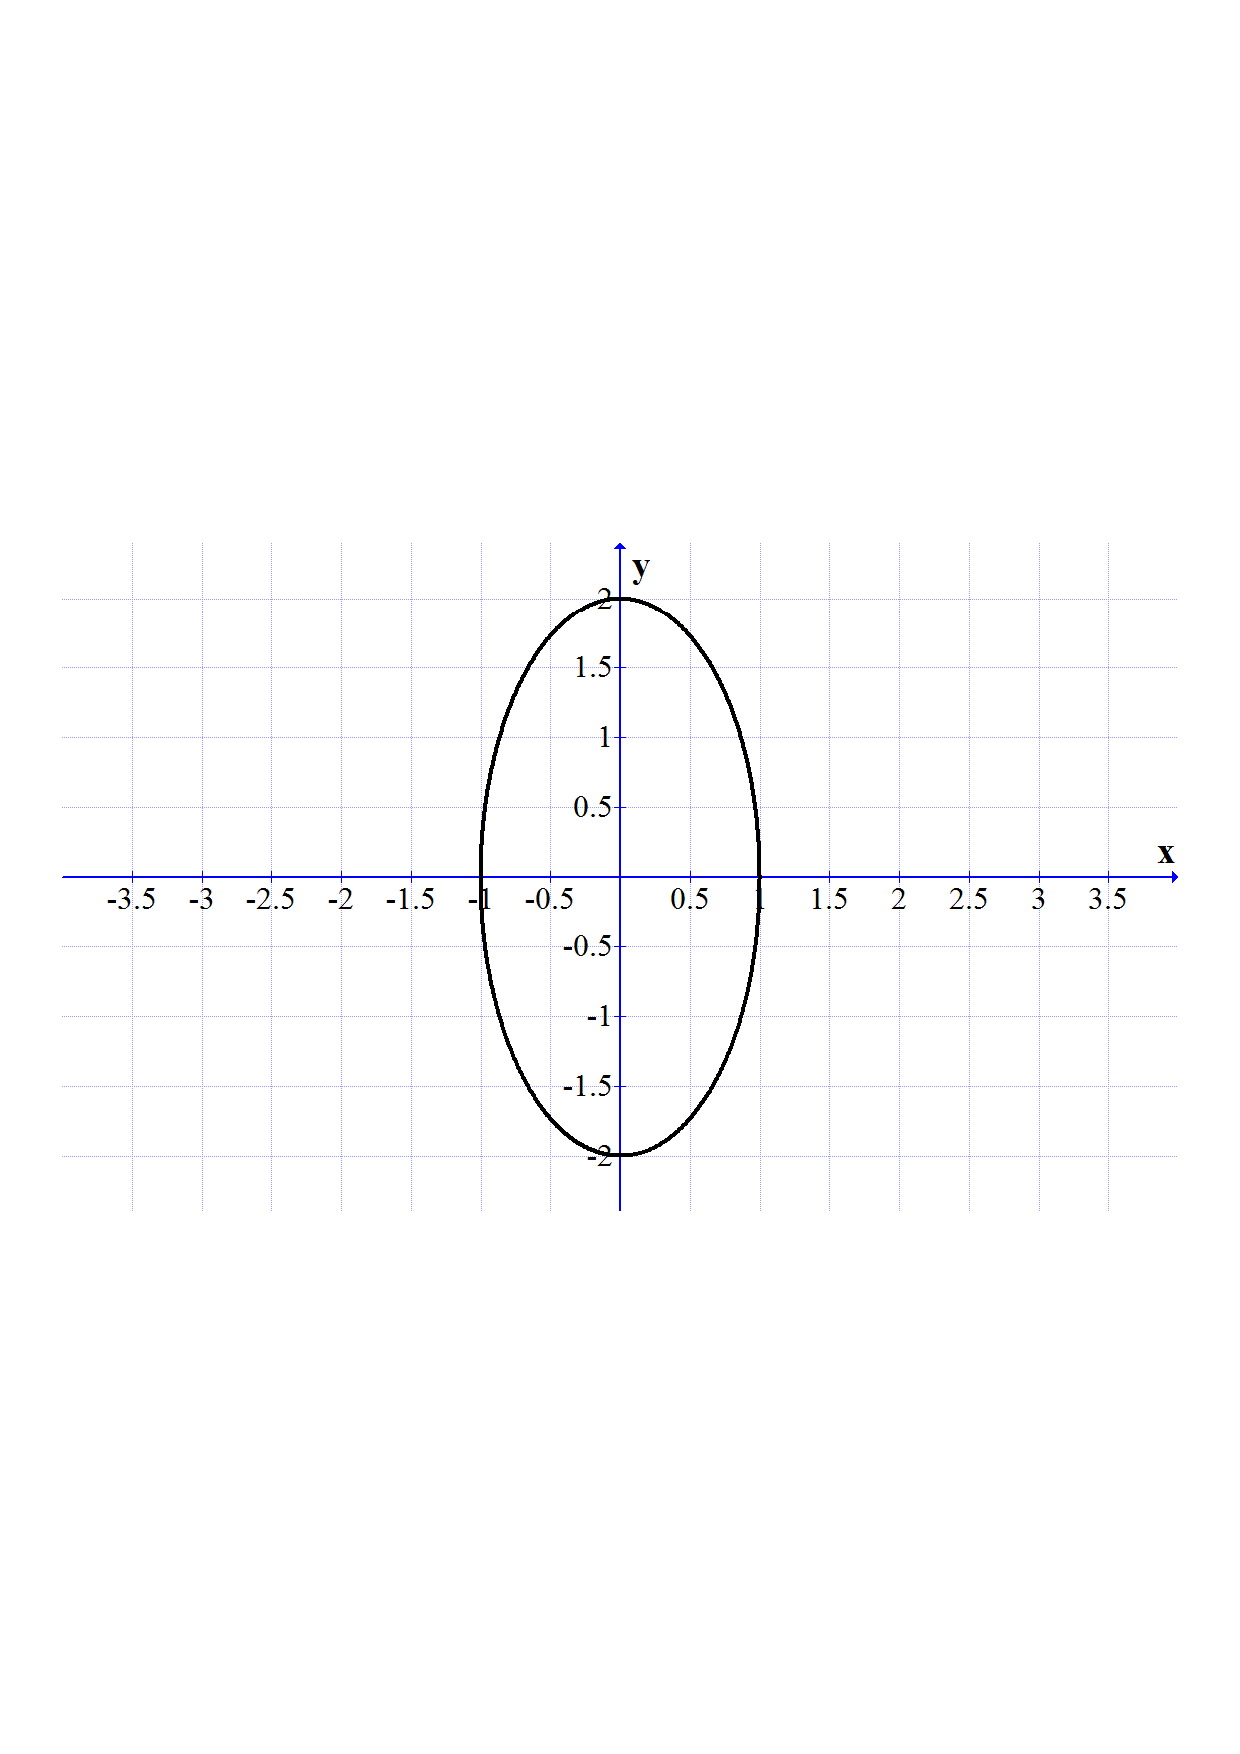
\includegraphics[scale=0.35]{LC2.pdf} & & 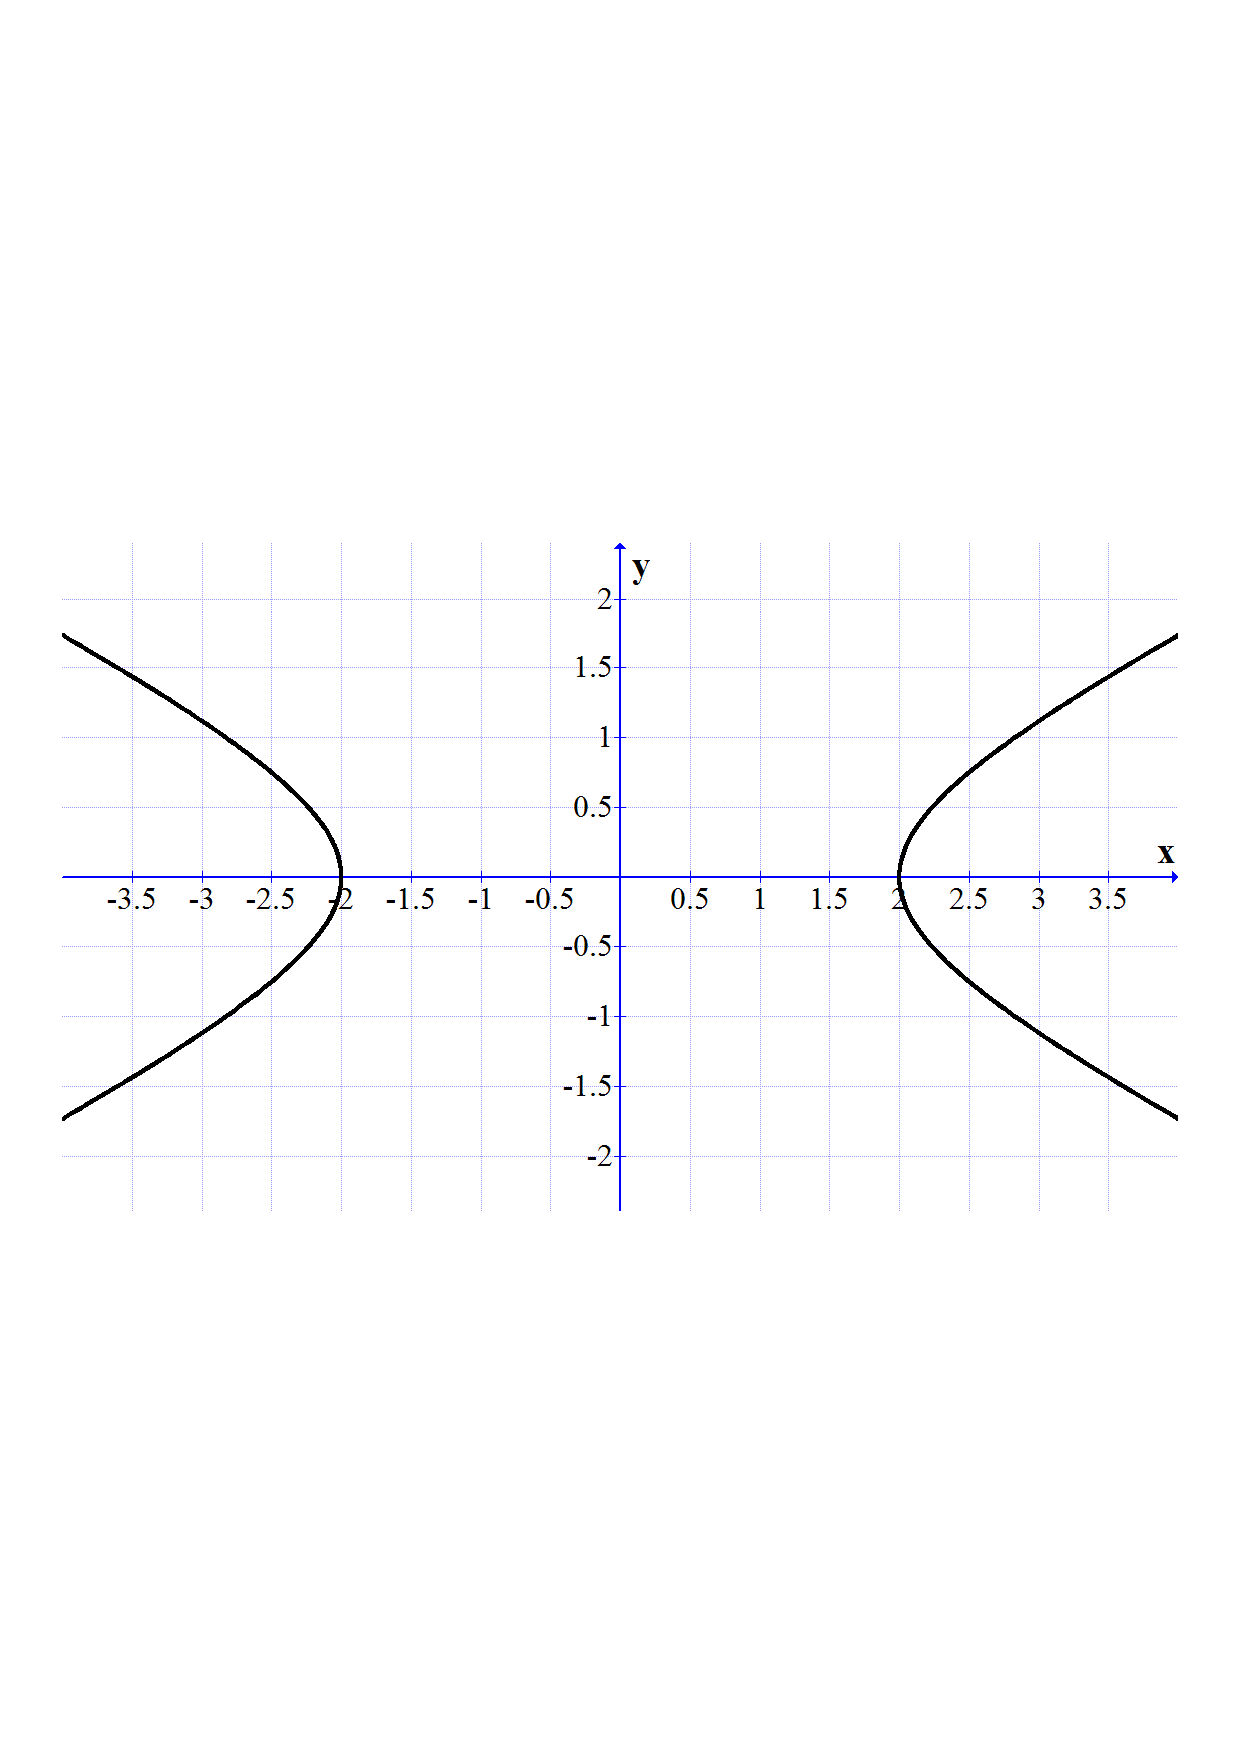
\includegraphics[scale=0.35]{LC5.pdf}\\
(c) & & & \\
&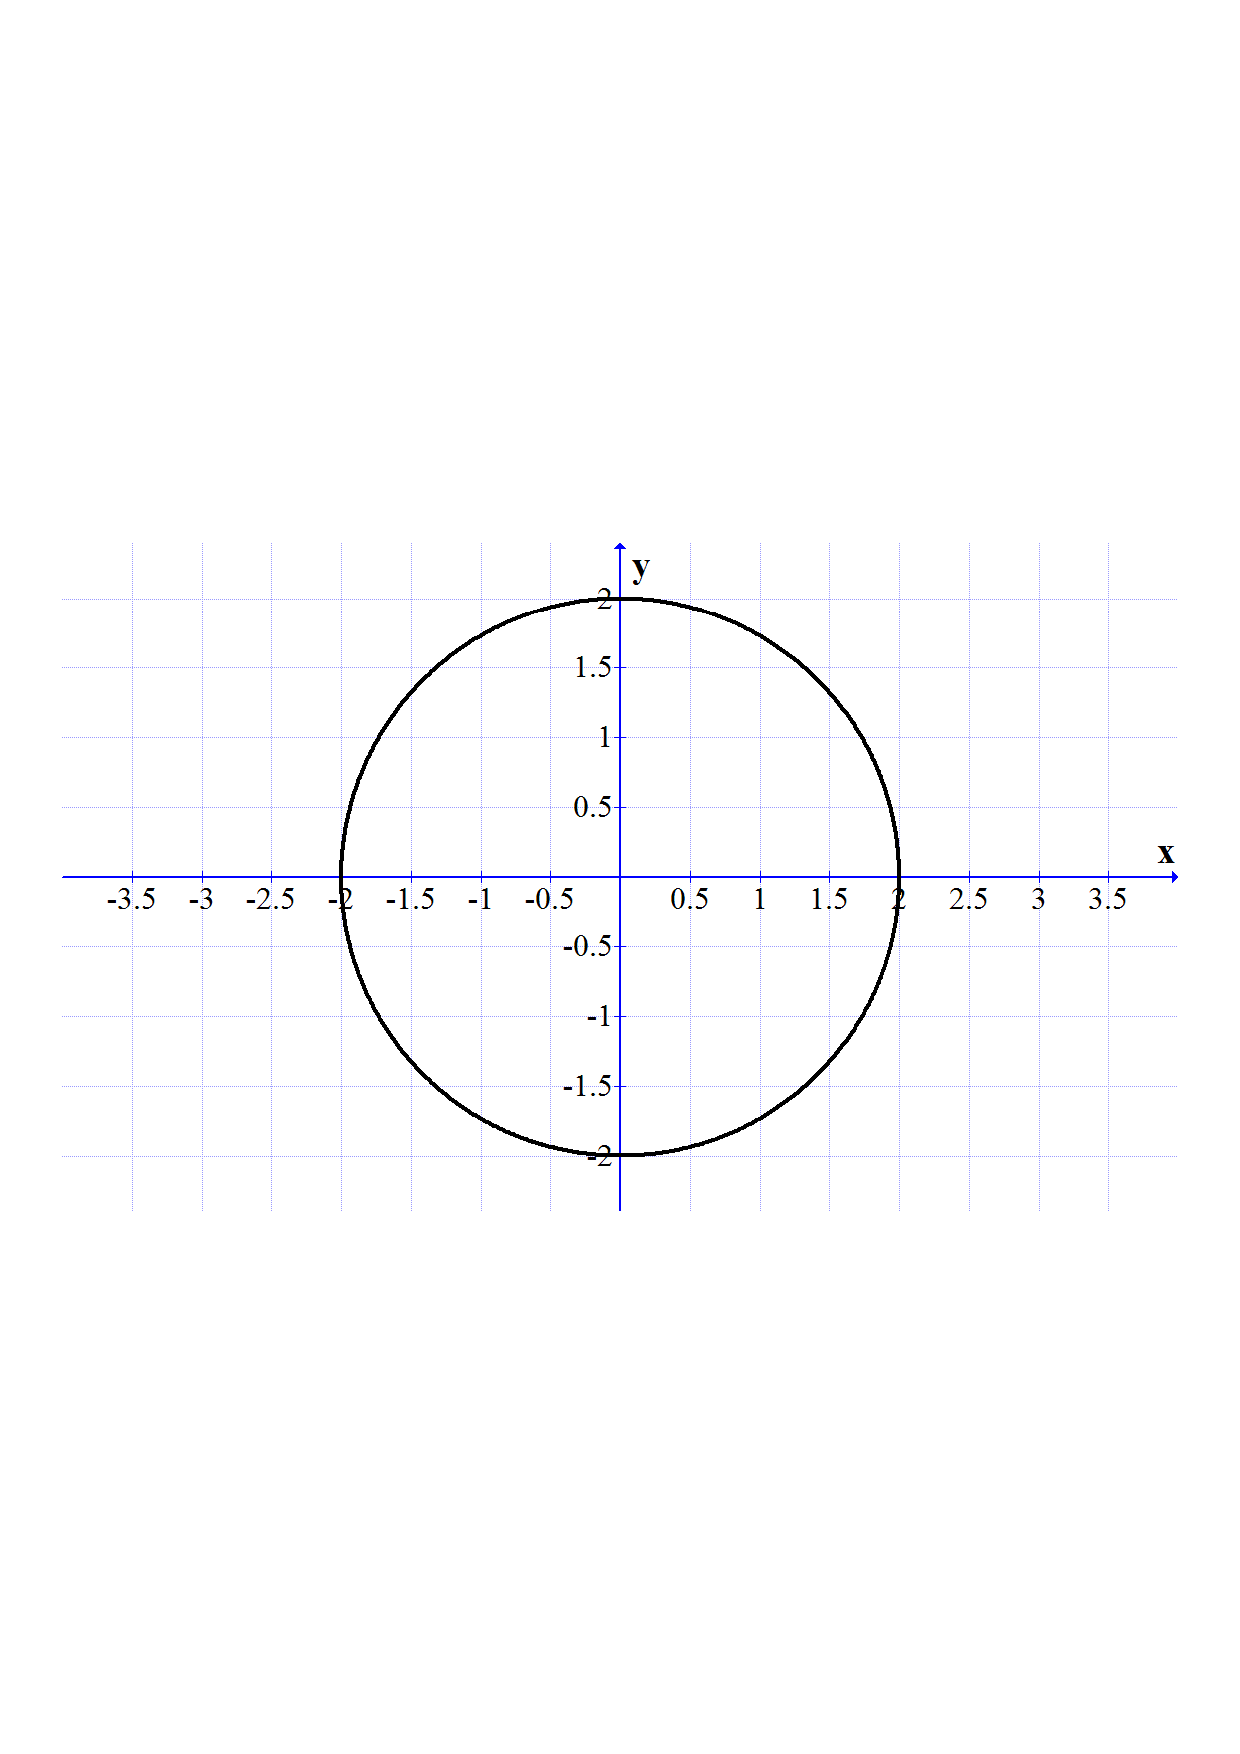
\includegraphics[scale=0.35]{LC3.pdf} & & 
\end{tabular}
\end{center}

\newpage

\item Suppose $f(x,y,z)=x^2+y^2-z^2$. For each of the following, sketch the level surface $f(x,y,z)=k$ corresponding to the indicated value of $k$.

\begin{enumerate}

\item $k=1$

\includegraphics[scale=0.5]{start.pdf}
{{{0.7\linewidth}{\begin{center}
$x^2+y^2-z^2=1$ is a hyperboloid of 1 sheet.\\
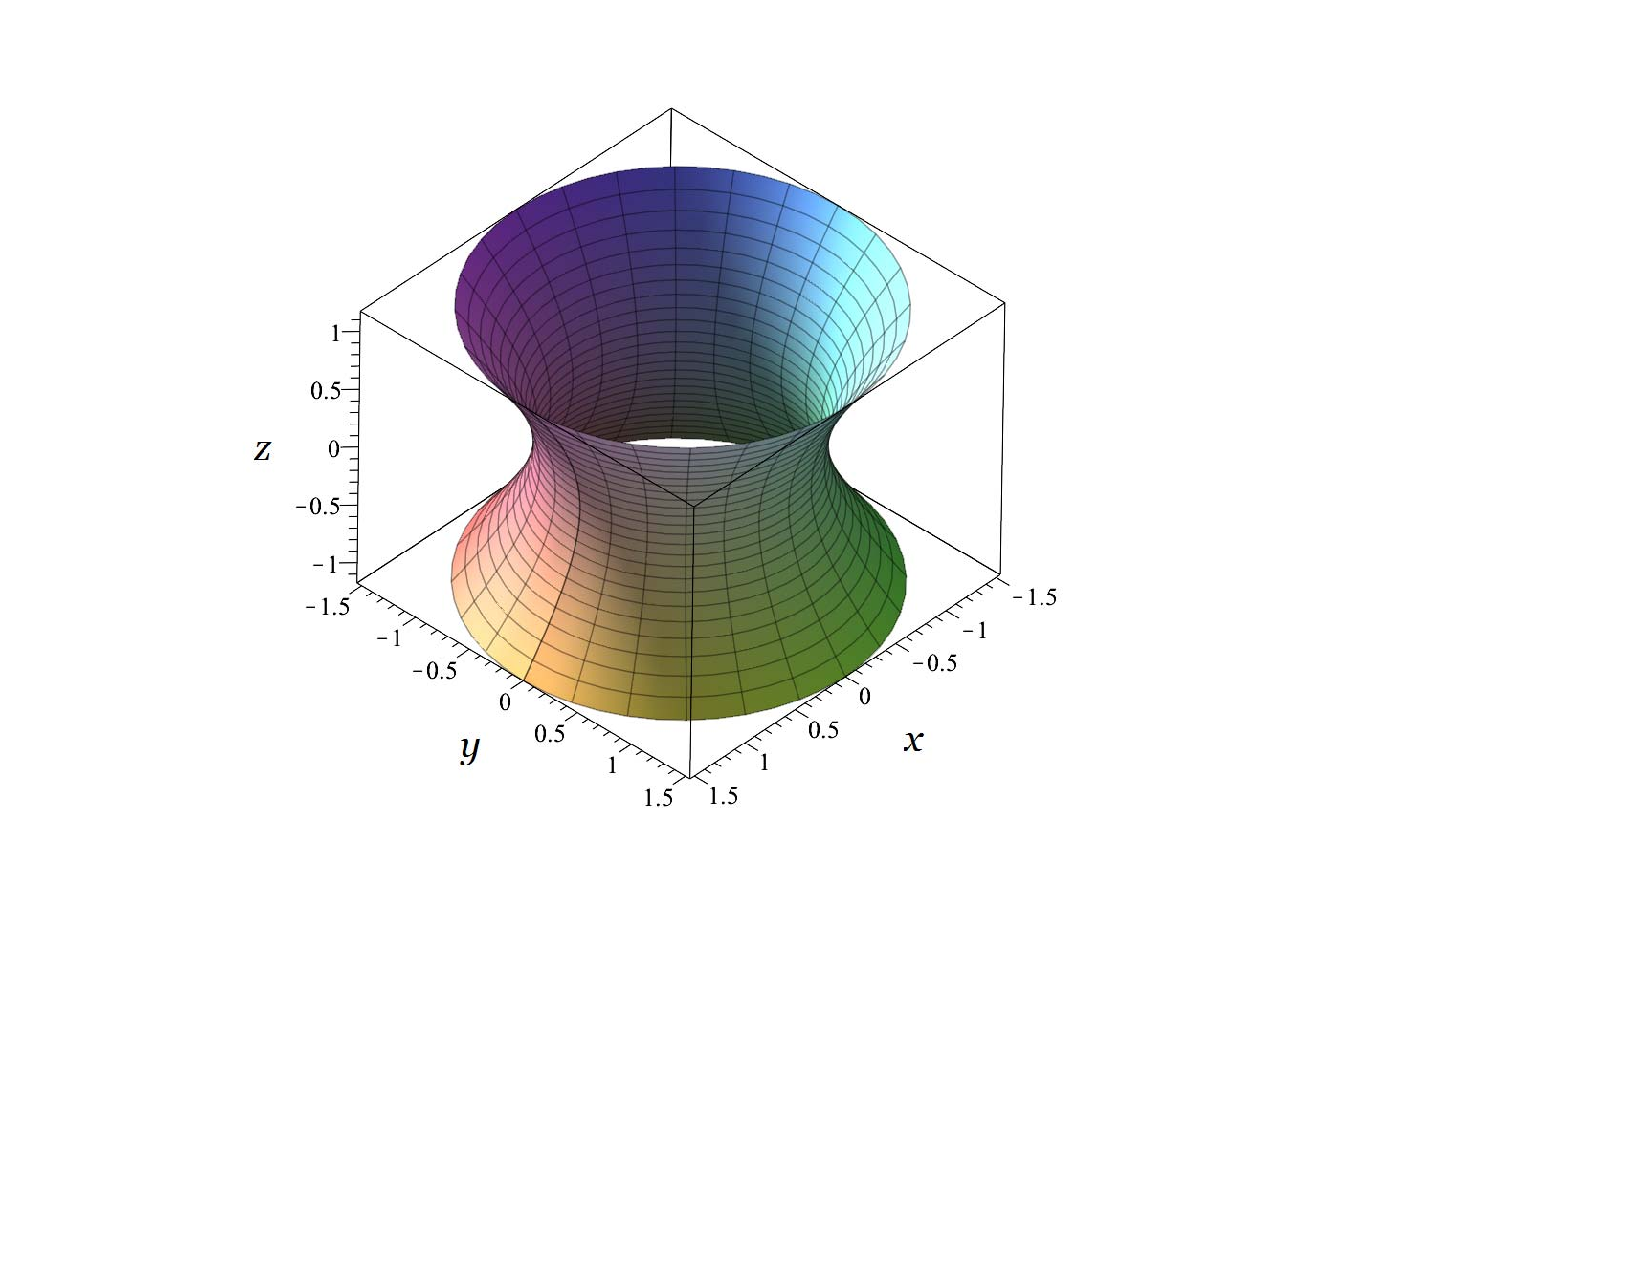
\includegraphics[scale=0.35]{hyperboloid1.pdf}
\end{center}}}}
\includegraphics[scale=0.5]{end.pdf}


\item $k=0$

\includegraphics[scale=0.5]{start.pdf}
{{{0.7\linewidth}{\begin{center}
$x^2+y^2=z^2$ is a double cone.\\
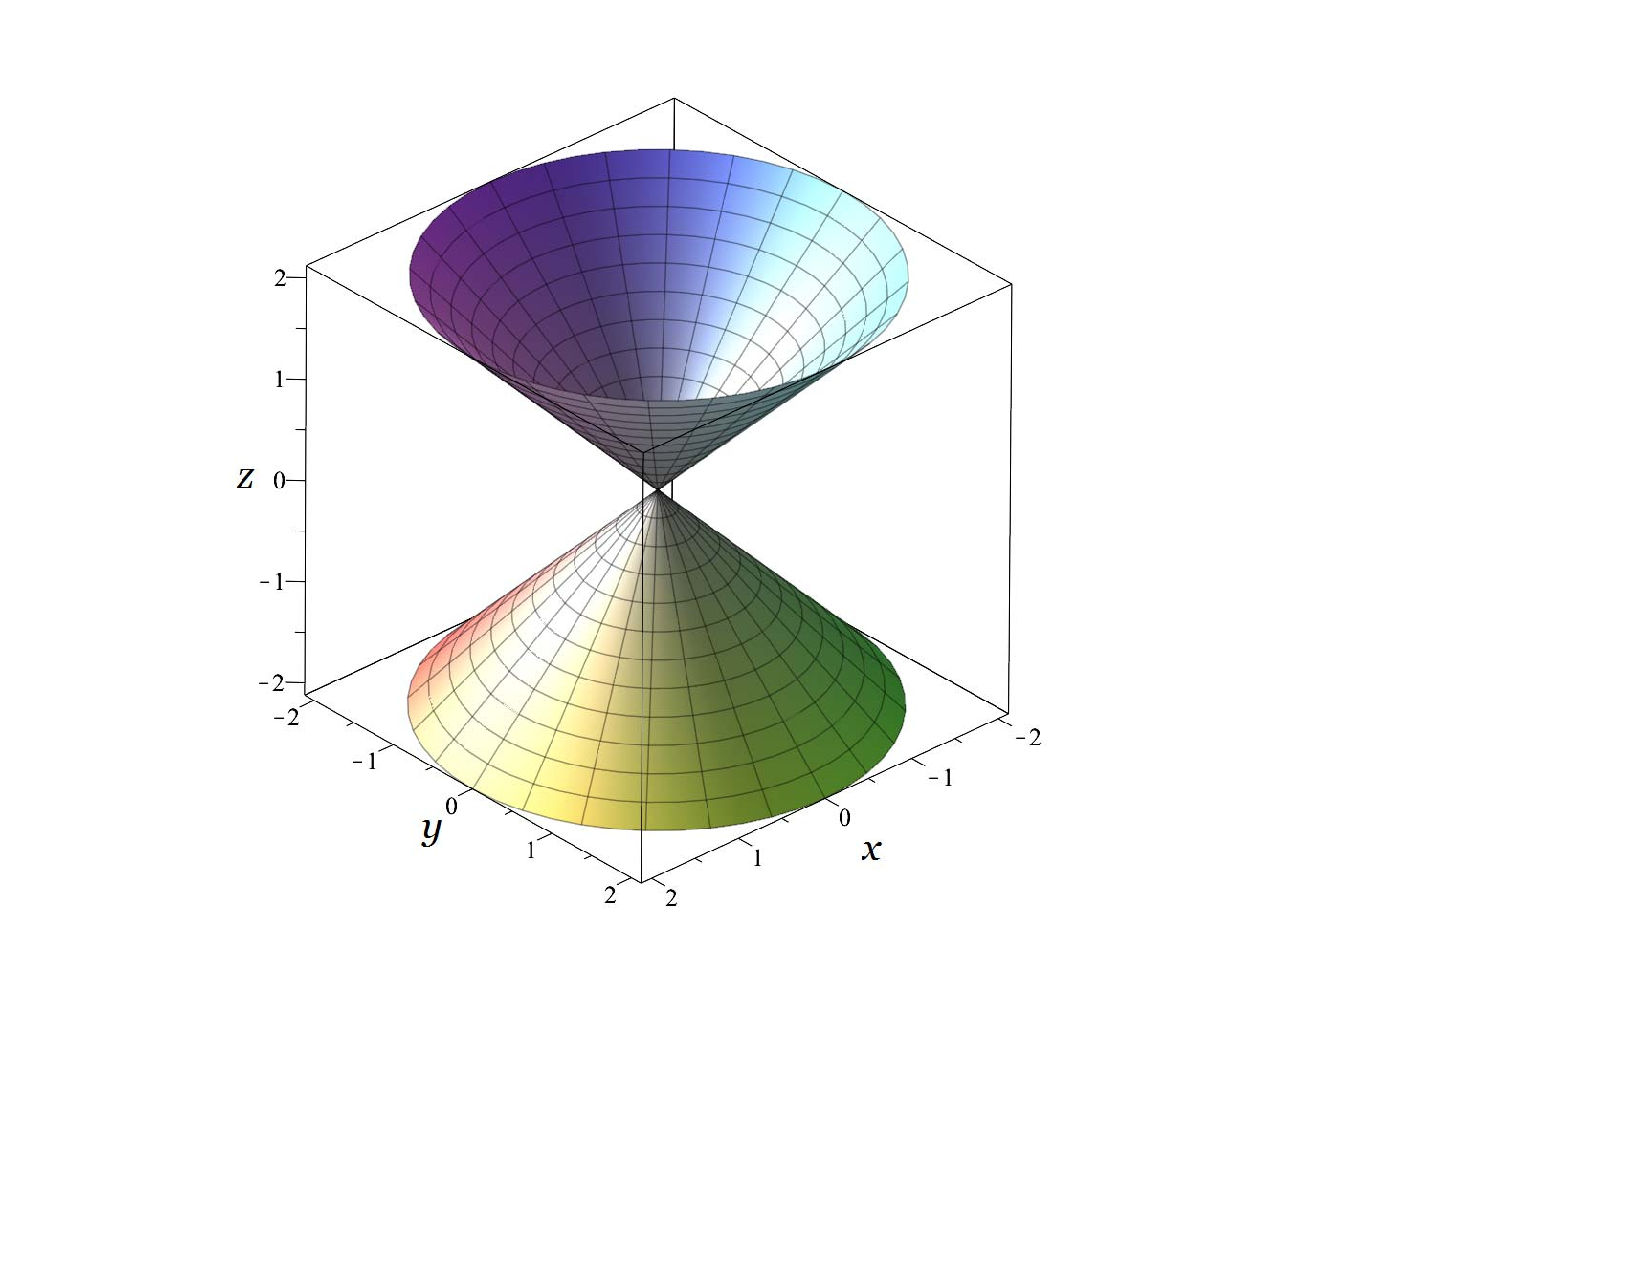
\includegraphics[scale=0.35]{cone.pdf}
\end{center}}}}
\includegraphics[scale=0.5]{end.pdf}


\item $k=-1$

\includegraphics[scale=0.5]{start.pdf}
{{{0.7\linewidth}{\begin{center}
$-x^2-y^2+z^2=1$ is a hyperboloid of 2 sheets.\\
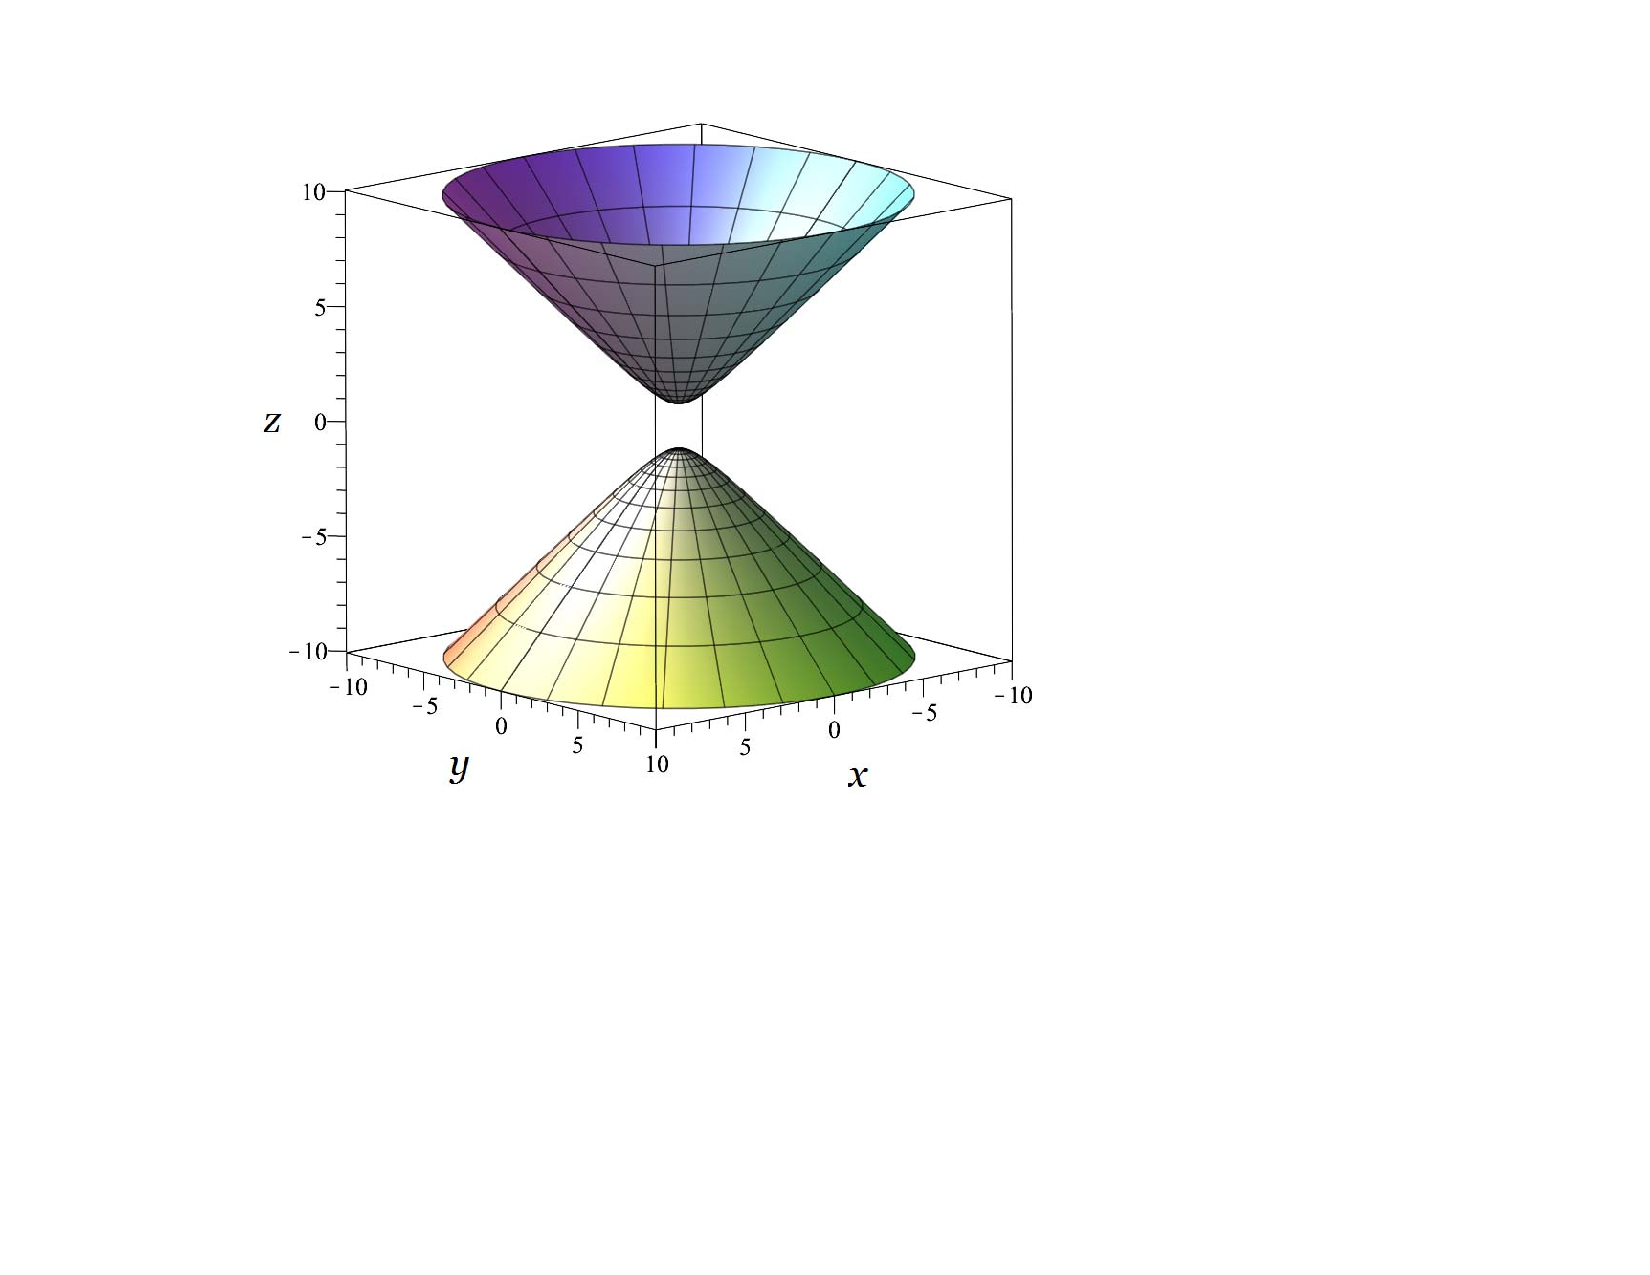
\includegraphics[scale=0.35]{hyperboloid2.pdf}
\end{center}}}}
\includegraphics[scale=0.5]{end.pdf}


\end{enumerate}

\item Consider the contour map shown below.

\begin{center}
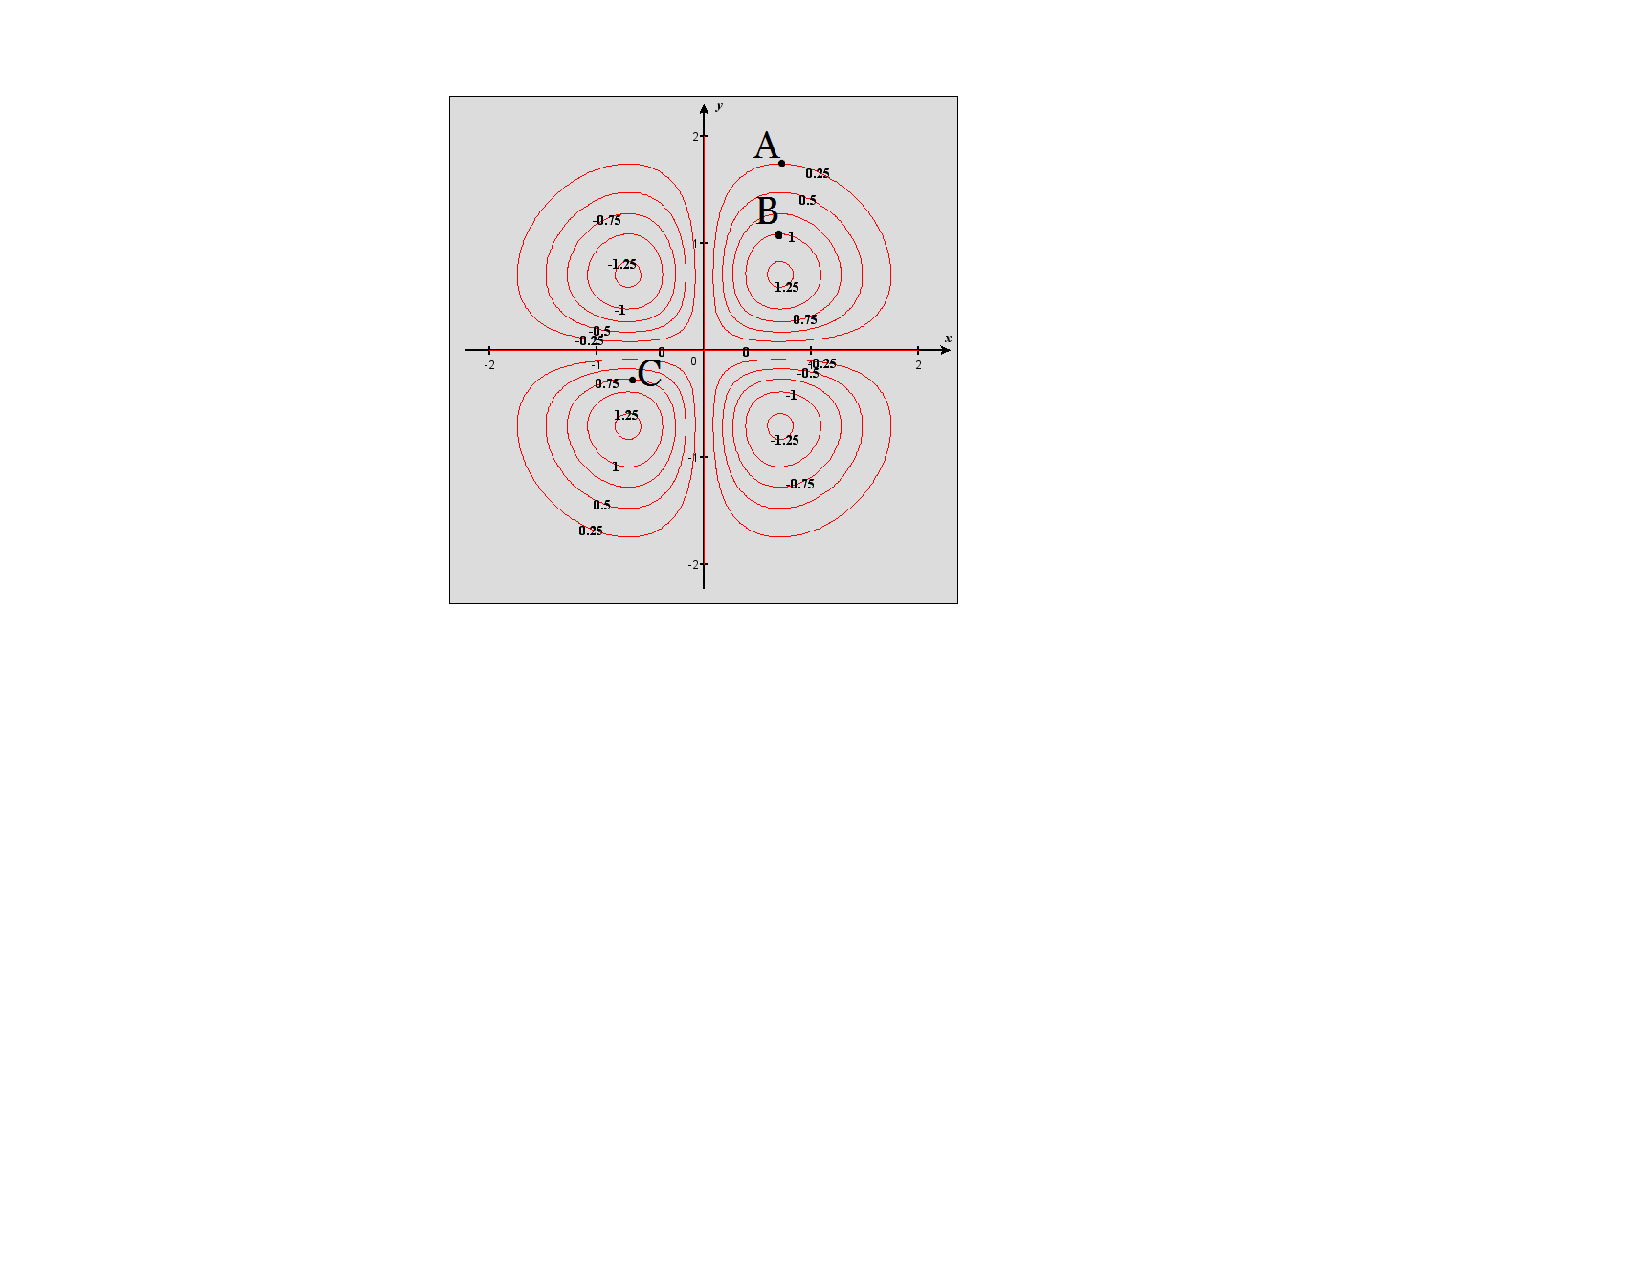
\includegraphics[scale=1]{contour.pdf}
\end{center}

\begin{enumerate}

\item If a person were walking straight from point $A$ to point $B$, would s/he be walking uphill or downhill?

\includegraphics[scale=0.5]{start.pdf}
{{Uphill}}
\includegraphics[scale=0.5]{end.pdf}


\item Is the slope steeper at point $B$ or point $C$?

\includegraphics[scale=0.5]{start.pdf}
{{Point $C$}}
\includegraphics[scale=0.5]{end.pdf}


\item Starting at $C$ and moving so that $x$ remains contant and $y$ decreases, will the elevation begin to increase or decrease?

\includegraphics[scale=0.5]{start.pdf}
{{Increase}}
\includegraphics[scale=0.5]{end.pdf}


\item Starting at $B$ and moving so that $y$ remains contant and $x$ increases, will the elevation begin to increase or decrease?

\includegraphics[scale=0.5]{start.pdf}
{{Decrease}}
\includegraphics[scale=0.5]{end.pdf}


\end{enumerate}

\newpage

\item {\bf Matching:} Each of the following contour plots were drawn on the window $[-3,3]\times[-3,3]$ in the $xy$-plane.  Points with larger $z$-values are shaded in blue.  Those with smaller $z$-values are shaded in red.  Match each contour map (a-f) to an appropriate graph (I-VI).

\begin{center}
\begin{tabular}{lc|cc}
(a)&&(d)\\
&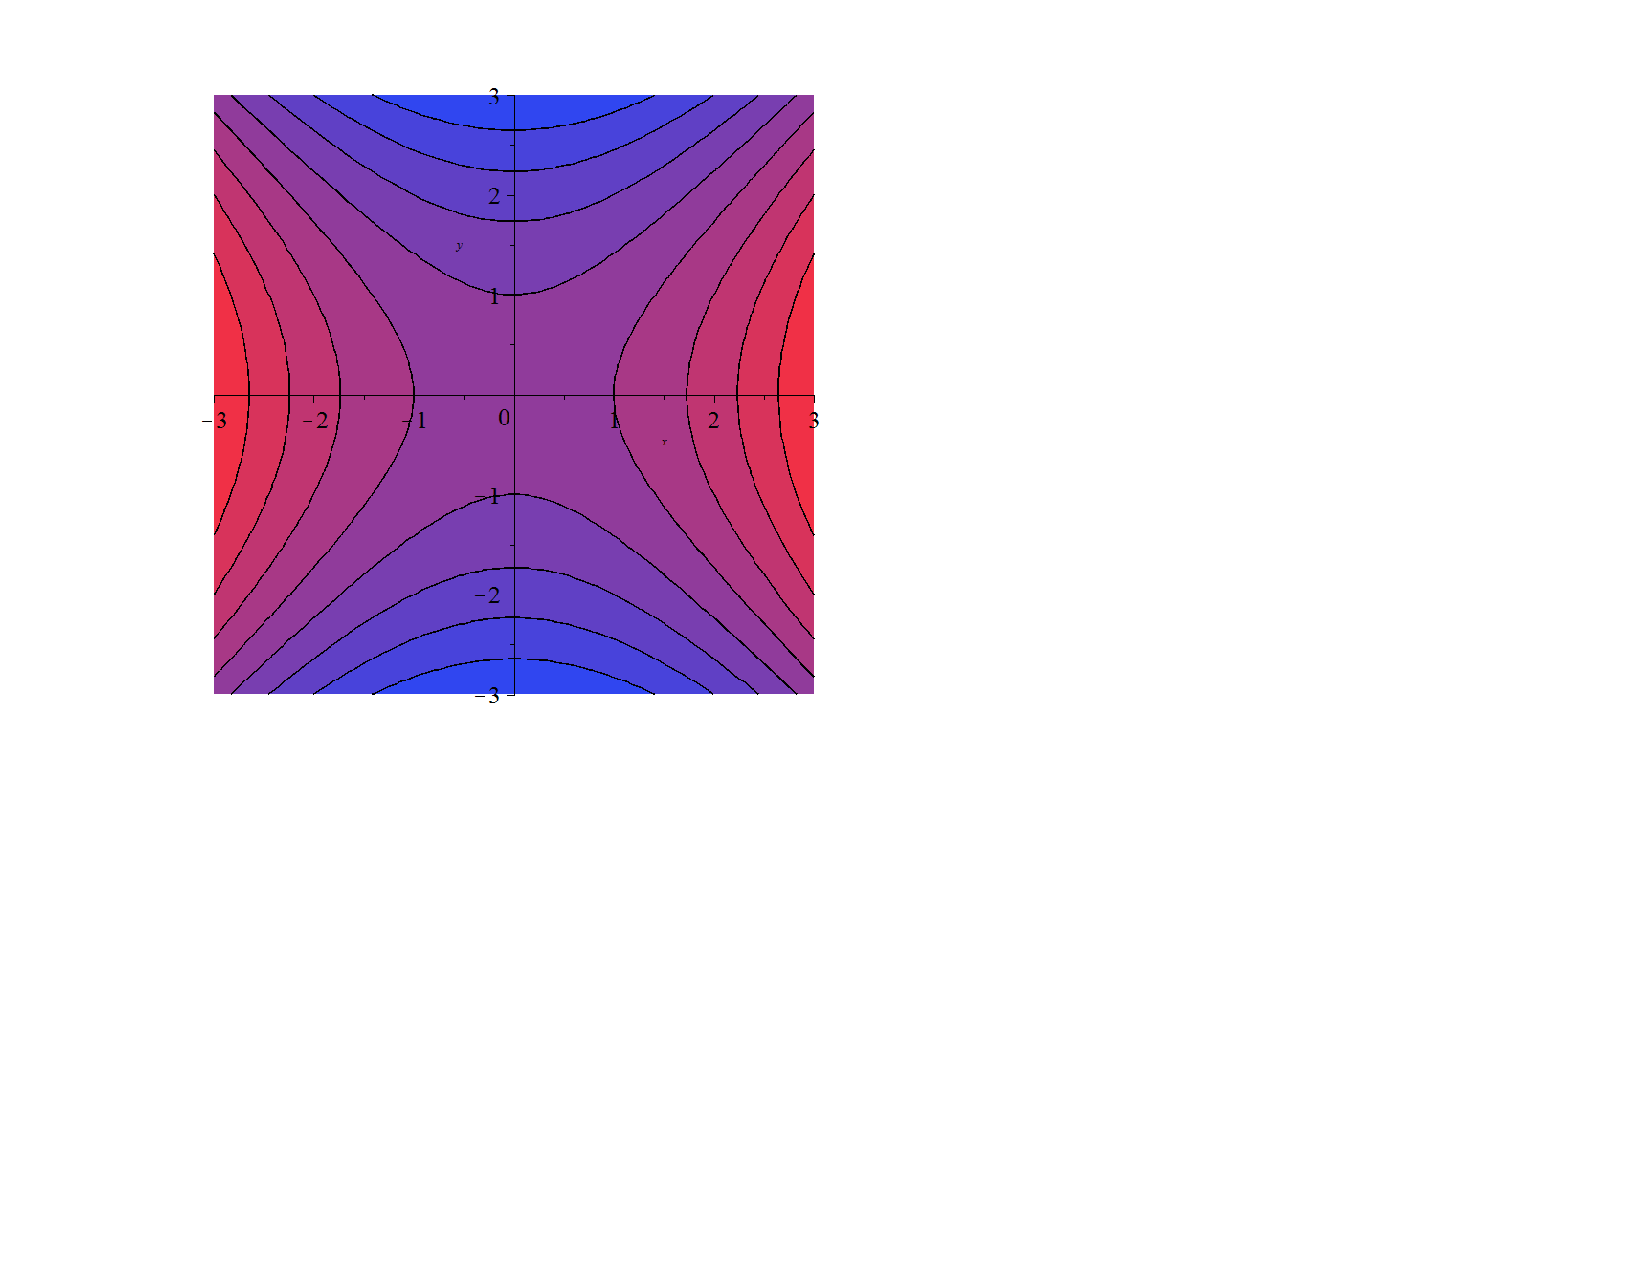
\includegraphics[scale=0.52]{matching1.pdf} &\hspace{0.5 cm}& 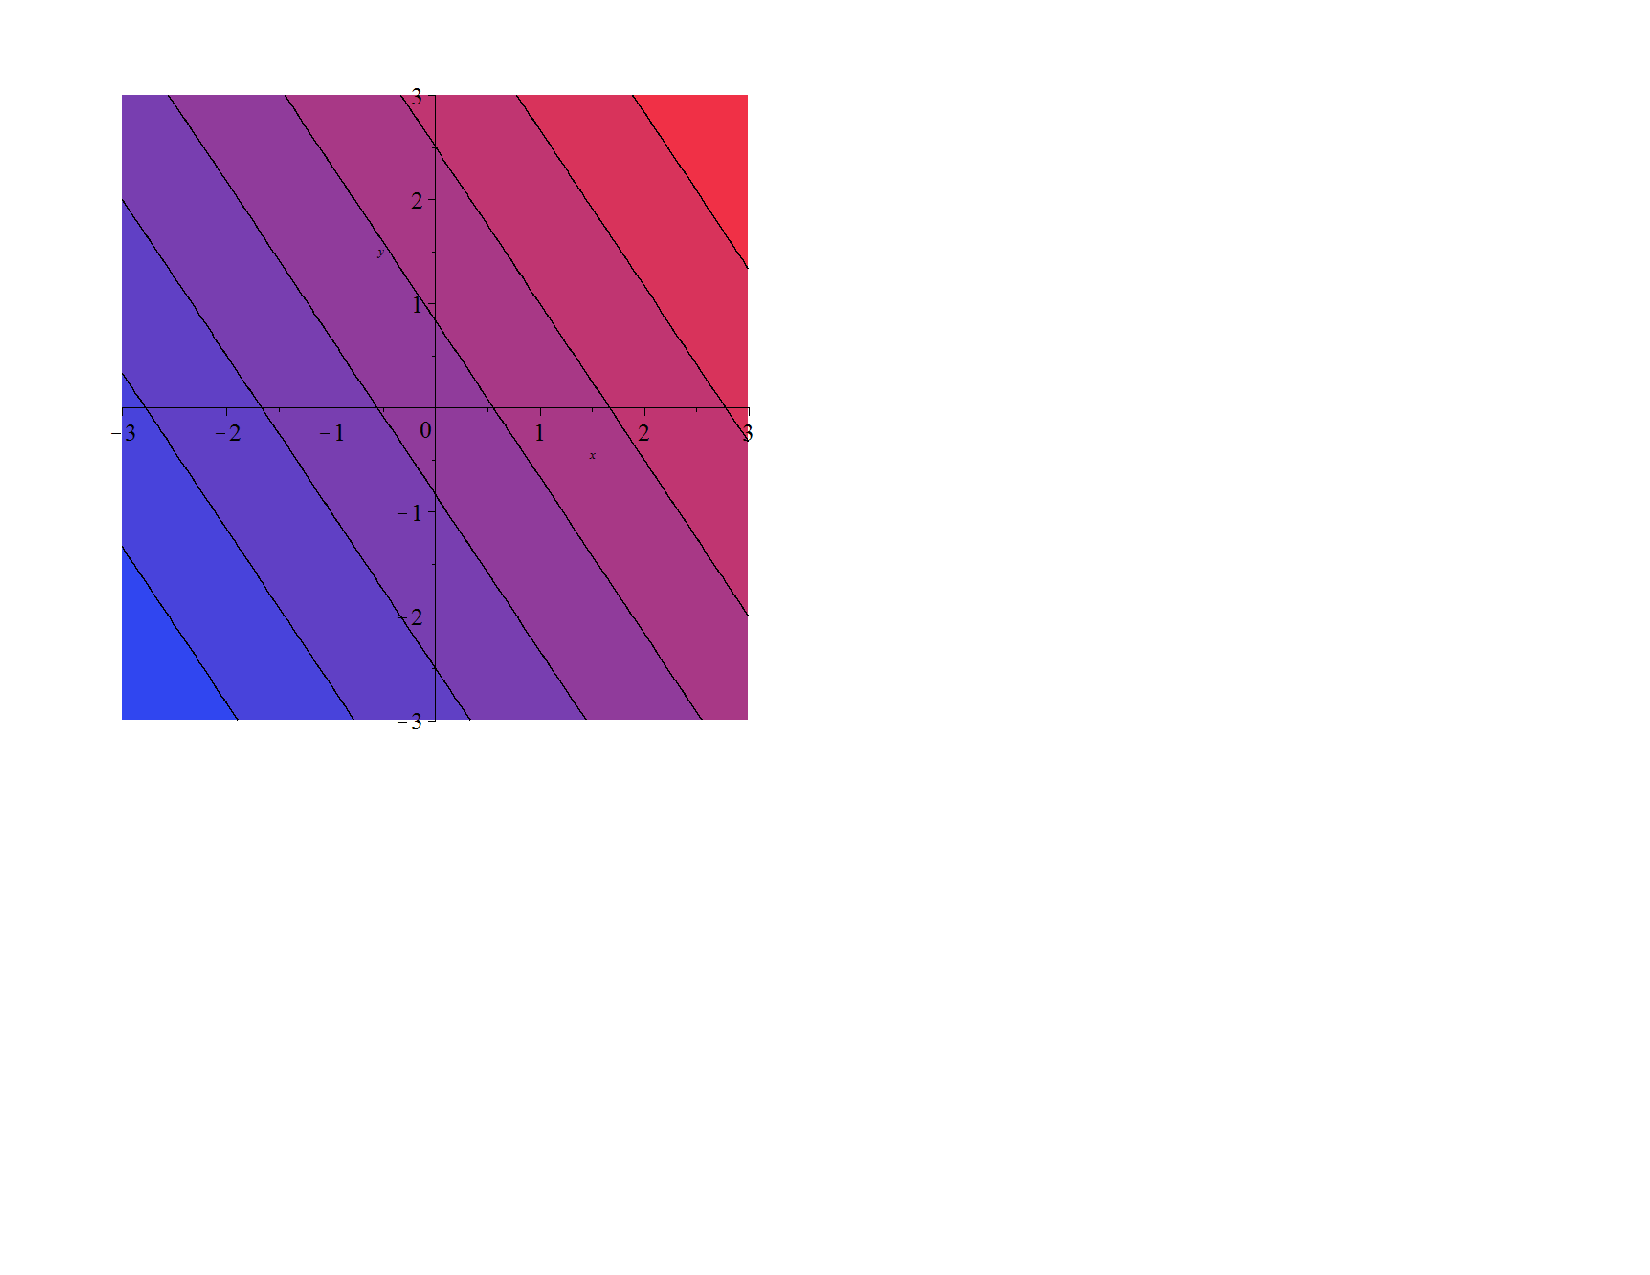
\includegraphics[scale=0.5]{matching4.pdf}\\
(b)&&(e)\\
&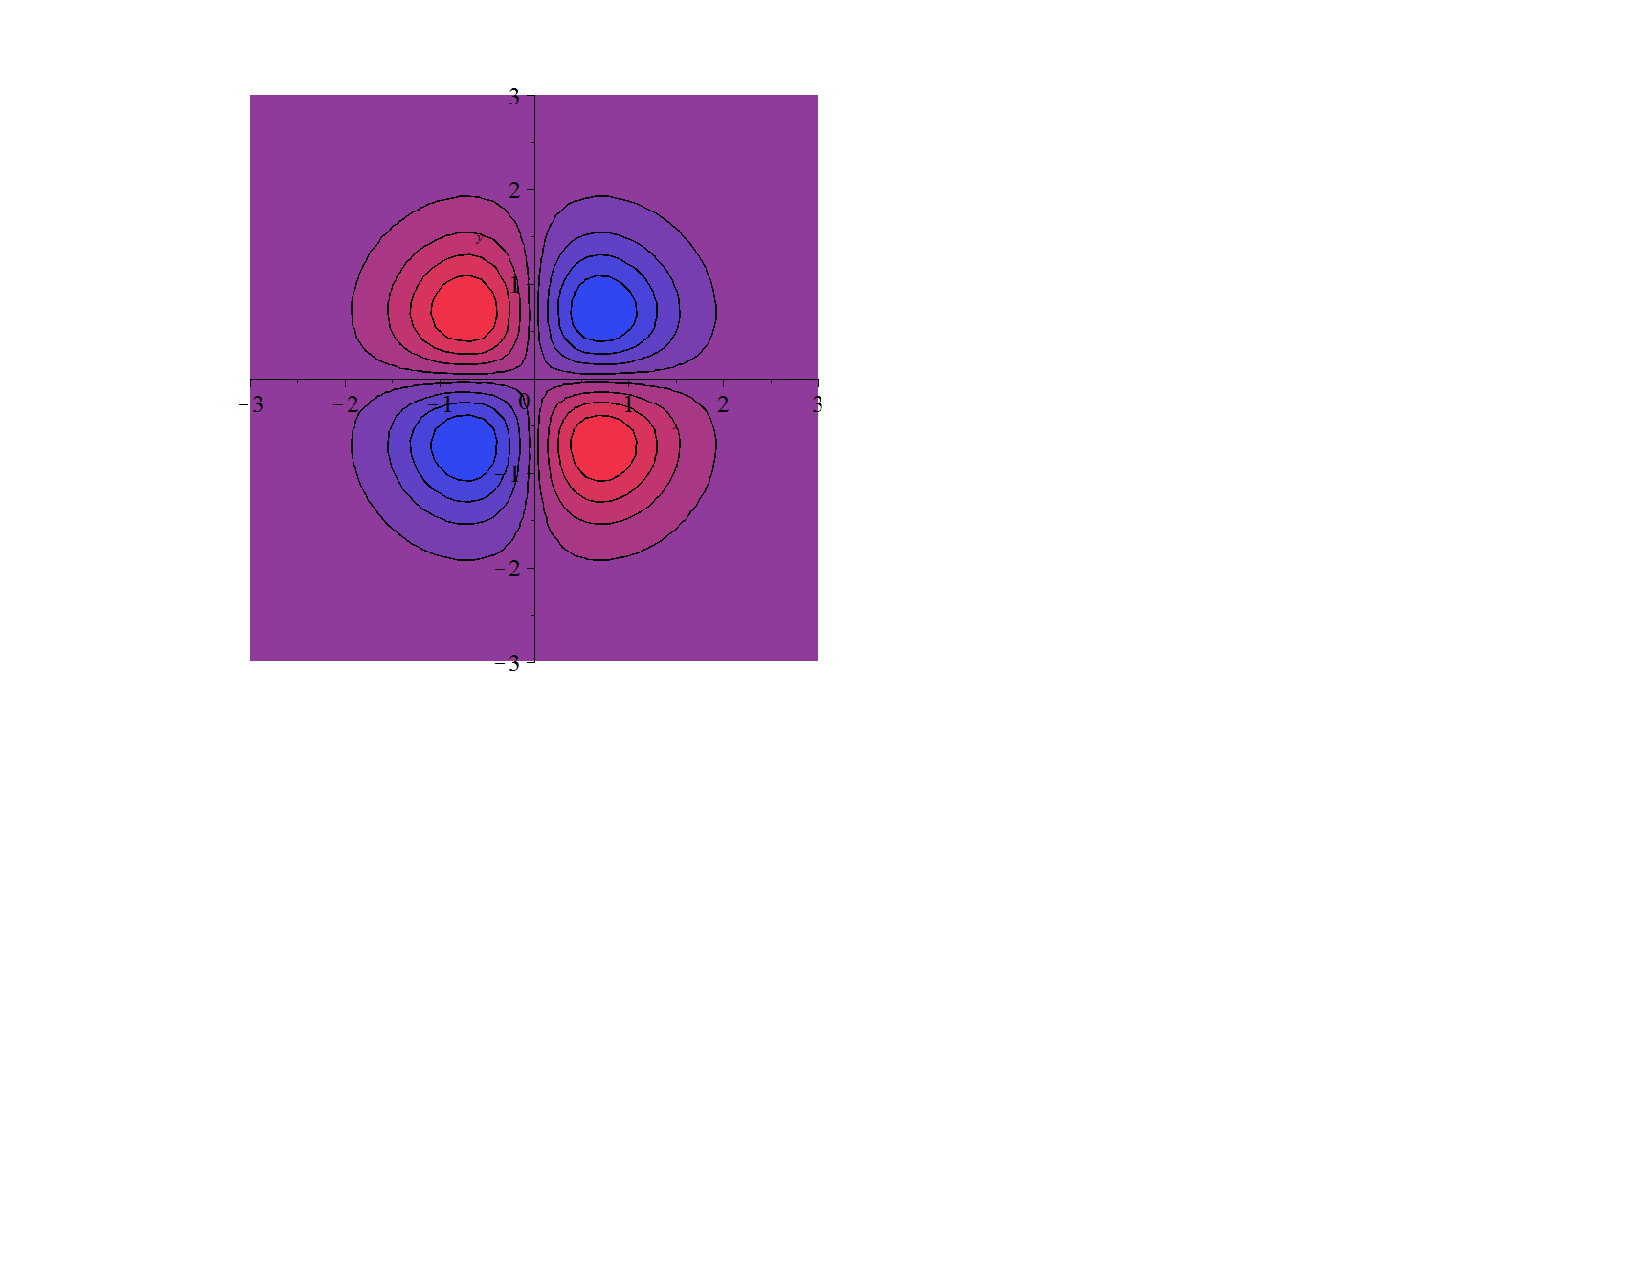
\includegraphics[scale=0.56]{matching2.pdf} && 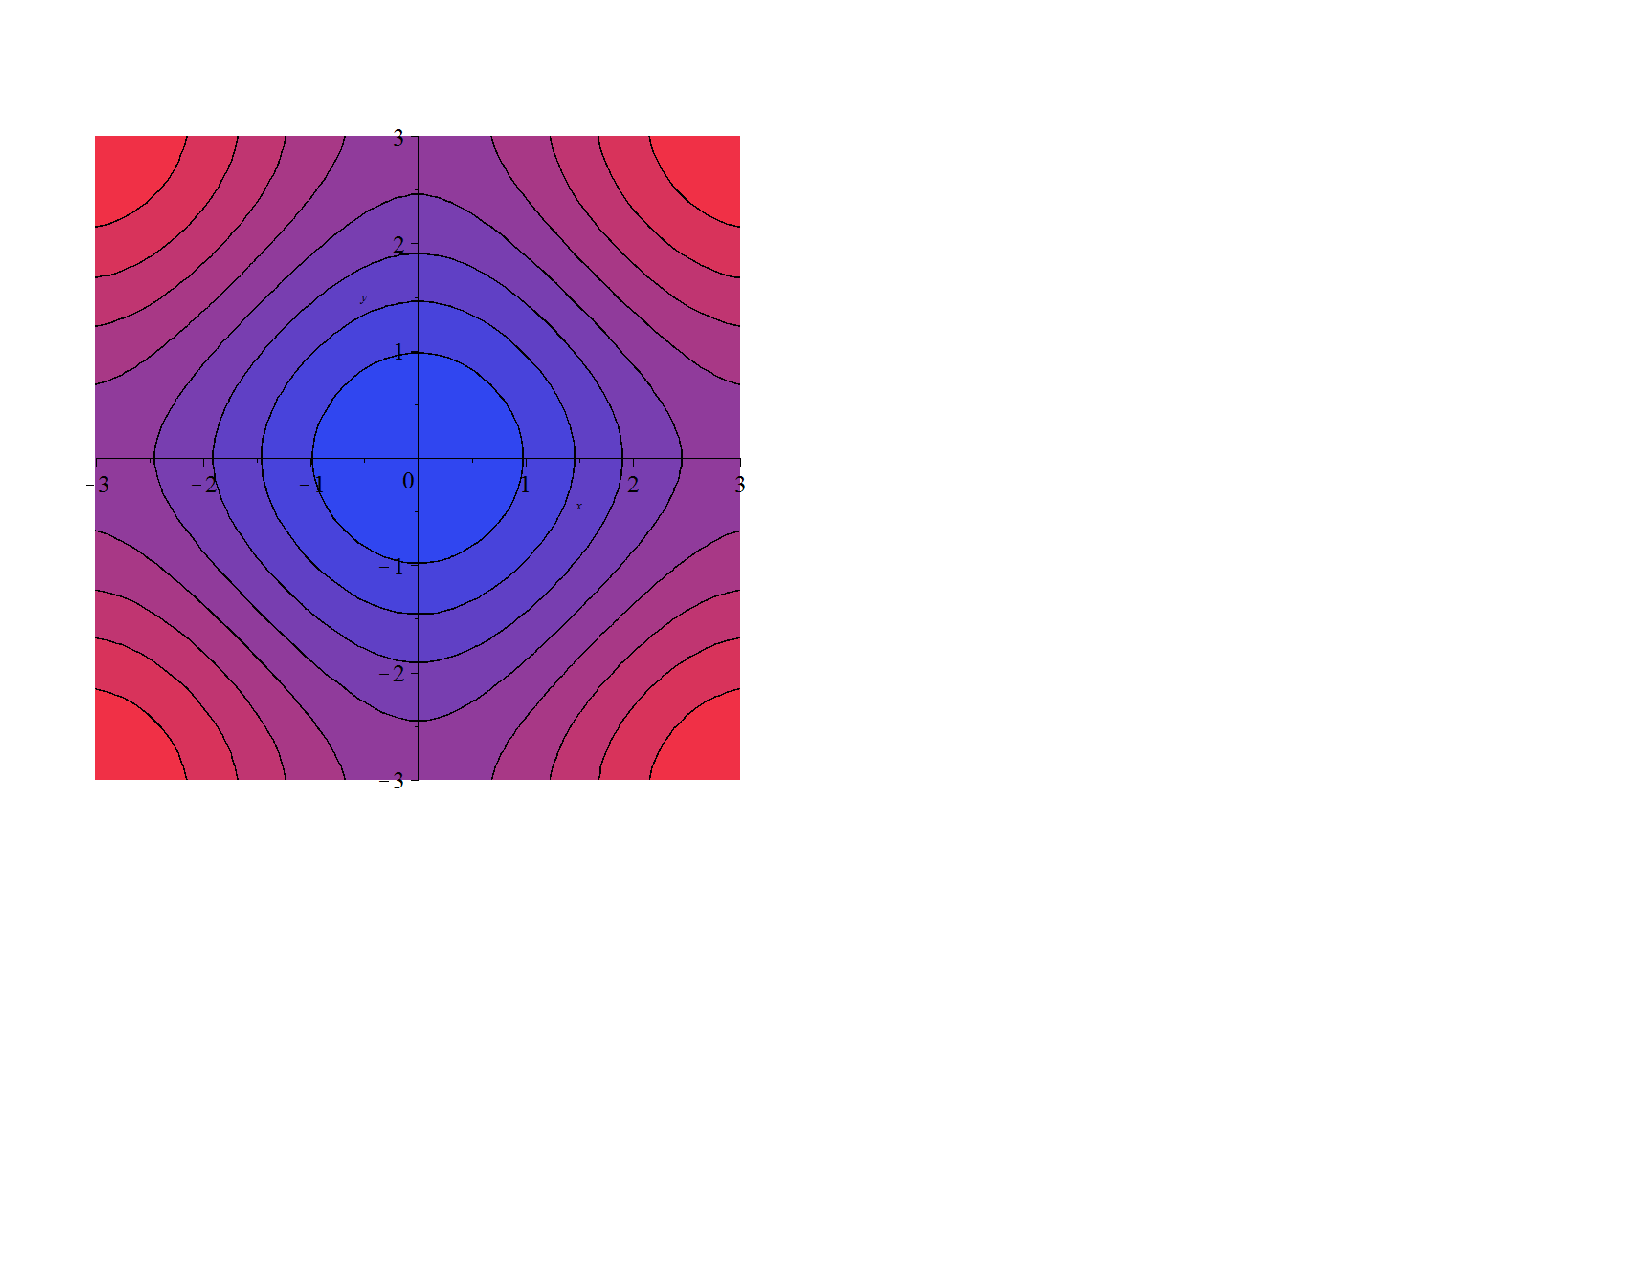
\includegraphics[scale=0.48]{matching5.pdf}\\
(c)&&(f)\\
&\includegraphics[scale=0.45]{matching3.pdf} && \includegraphics[scale=0.49]{matching6.pdf}
\end{tabular}
\end{center}

\newpage

\begin{center}
\begin{tabular}{lc|cc}
(I)&&(IV)\\
&\includegraphics[scale=0.45]{matchinge.pdf} &\hspace{0.5 cm}& \includegraphics[scale=0.5]{matchingb.pdf}\\
(II)&&(V)\\
&\includegraphics[scale=0.5]{matchingd.pdf} && \includegraphics[scale=0.5]{matchinga.pdf}\\
(III)&&(VI)\\
&\includegraphics[scale=0.45]{matchingf.pdf} && \includegraphics[scale=0.45]{matchingc.pdf}
\end{tabular}
\end{center}

\newpage

\includegraphics[scale=0.5]{start.pdf}
{{{0.35\linewidth}{\begin{center}\begin{tabular}{c|c}
{\bf Contour Plot} & {\bf Graph}\\
\hline
a & V\\
b & IV\\
c & VI\\
d & III\\
e & II\\
f & I
\end{tabular}\end{center}}}}
\includegraphics[scale=0.5]{end.pdf}


\item {\bf Multiple Choice:} Which of the following is a sketch of the domain of $\displaystyle f(x,y)=\ln{(xy-1)}+e^{x^{2}y}-y^{8}$?

\begin{tabular}{lll}
(a) & \text{ }\text{ } & (d)\\
\includegraphics[scale=0.35]{D1.pdf} & & \includegraphics[scale=0.35]{D4.pdf}\\
(b) & \text{ }\text{ } & (e)\\
\includegraphics[scale=0.35]{D2.pdf} & & \includegraphics[scale=0.35]{D5.pdf}\\
(c) & & \\
\includegraphics[scale=0.35]{D3.pdf} & & 
\end{tabular}

\includegraphics[scale=0.5]{start.pdf}
{{(a)}}
\includegraphics[scale=0.5]{end.pdf}


\item Suppose that $f(x,y)=x^2+y^2$.  And, consider line $L$ with parametric equations: $x(t)= \frac{\sqrt{2}}{2}t$, $y(t)=\frac{\sqrt{2}}{2}t$, $z(t)=0$.\\

Notice that this line in the $xy$-plane is parallel to the unit vector $\overrightarrow{u}= \left\langle \frac{\sqrt{2}}{2},\frac{\sqrt{2}}{2},0 \right \rangle$.

\begin{enumerate}

\item Now consider the image below.  The red curve along $f(x,y)$ is the curve that results from evaluating the function at points along $L$.  In other words, it is $f(x(t),y(t))$, where $x(t)$ and $y(t)$ are taken from the parametric equations of $L$.  Compute $f(x(t),y(t))$.

\begin{center}
\includegraphics[scale=0.5]{directional.pdf}
\end{center}

\includegraphics[scale=0.5]{start.pdf}
{{$f(x(t),y(t))=f\left(\frac{\sqrt{2}}{2}t,\frac{\sqrt{2}}{2}t\right)=t^2$}}
\includegraphics[scale=0.5]{end.pdf}


\item Notice that your answer from part (a) is a single variable function of the variable $t$.  Call it $g(t)$.  Compute $\left.\frac{d}{dt}\left(g(t)\right)\right|_{t=1}$ and interpret your answer geometrically.

\includegraphics[scale=0.5]{start.pdf}
{{{1\linewidth}{$\left.\frac{d}{dt}\left(g(t)\right)\right|_{t=1}=2$.  This can be thought of as the instantaneous rate of change of $f(x,y)=x^2+y^2$ at the point $(x,y,z)=\left(\frac{\sqrt{2}}{2}, \frac{\sqrt{2}}{2},1\right)$ in the direction of $\overrightarrow{u}$; or, equivalently, this can be thought of the slope of the tangent line to the red curve on the surface at the point $(x,y,z)=\left(\frac{\sqrt{2}}{2}, \frac{\sqrt{2}}{2}, 1\right)$.}}}
\includegraphics[scale=0.5]{end.pdf}


\end{enumerate}

\end{enumerate}

\end{document}